\chapter{Long-Term Autonomous Mobile Robots}
\label{sec:lta_mobile_robots}

Long-term autonomous mobile robotic systems can be of great benefit in diverse environments. For the most part, in activities that are either too dangerous
or too undemanding (monotonous, not meaningful) to be performed by humans. In addition, economic considerations may play a role, as well as tasks 
that are undesirable for other reasons.
All three attributes - \textit{long-term}, \textit{autonomous}, and \textit{mobile} - have the potential of dramatically increasing the complexity and
the risk for failures of the system. Part of this chapter will be to precisely define what each of the attributes means in the context of this work.
The attribute of mobility is the easiest to define: A mobile robot is a system capable of moving freely (within limits) through an environment. \cite{Hertzberg:2012}
Thus, it's about the ability of a robot to move rather than being statically attached to a position.\newline
First, an extensive literature review is given in section \ref{sec:literature_review} to provide a meaningful overview of the state of the art.
Afterwards, section \ref{sec:lta_plant_observation} introduces the scenario that is going to be studied in this work and provides a definition for the concept of long-term
autonomy as understood in the following chapters, i.e., clarifies what the two remaining attributes \textit{long-term} and \textit{autonomous} are supposed to mean.
Subsequently, the prototypical scenario in the simulation is explained in section \ref{sec:prototype_scenario}. Section \ref{sec:robotic_system} discusses the scientific and
technological background that forms the basis of this work. Finally, section \ref{sec:challenges_for_lta} identifies potential hinderances for long-term autonomous systems with
a particular focus on the considered plant monitoring scenario.

\section{Literature Review - State of the Art}
\label{sec:literature_review}

As the title of this thesis indicates, it addresses several research domains usually considered in isolation. First, there is the execution monitoring aspect, which is not only
concerned with potential problems for a robotic system (software / hardware), but also with environmental conditions that threaten the successful completion of a robot's mission.
In addition, the work focuses on the long-term autonomous application of mobile robotic systems in the context of plant monitoring. All of these aspects (long-term, autonomy,
mobility, plant monitoring) can be considered and researched in isolation, which is what has been done for all of these sub-areas. The aim of this work, however, is to examine all of
these aspects in combination and to focus on the big picture of integrating them into systems that are actually useful. The following literature review will therefore attempt to
provide a chronological overview of the literature on all of these subfields, but with the clear intention of considering them together rather than in isolation.
One distinction that must be emphasized when reviewing long-term autonomous robot applications in the literature is the distinction between indoor and outdoor environments.
So far, there has been a focus on indoor environments. \cite{Kyberd:2021} Despite the indisputable challenges that indoor environments pose, they are arguably less dangerous and
troublesome than outdoor scenarios. \cite{Hawes:2017} Considering the broadness of these research fields, it is obviously not possible to discuss all the relevant fundamentals.
The idea is to provide a meaningful overview, which sufficiently frames the present thesis.\newline

\noindent
\textit{Long-Term Autonomy}\newline

\noindent
Early examples of long-term autonomous mobile service robots are \textit{RHINO} (1998), an interactive museum tour guide developed by Burgard et al. \cite{Burgard:1998}
and its successor \textit{MINERVA} (1999) with improved navigation capabilities presented by Thrun et al. \cite{Thrun:1999}.
They focus on robust localization (pose estimation) and navigation in crowded environments, as well as viable human-robot interaction.\newline
The highly successful examples of \textit{RHINO} and \textit{MINERVA} were followed by numerous works on mobile indoor robots focusing on specific technological aspects of
meaningful autonomy in such environments.
Nourbakhsh et al. \cite{Nourbakhsh:2003} also consider the deployment of long-term autonomous mobile robots in a museum setting, considering in particular the aspect that
it is infeasible to place autonomous robots under full-time human supervision. They claim that, in any case, these robots should reach a level of autonomy that allows them to act
fully autonomously until they are confronted with a problem they cannot solve. In which case: \textquote{\textit{[...] critical aspect of autonomy in our unsupervised application
is the ability to detect failure and signal humans for help.}} \cite{Nourbakhsh:2003} The authors have already implemented some diagnostics and methods for responding to failure cases,
mainly based on the simple but effective idea of retrying a failed task. After an iterative process of testing and refining the diagnostics over a long period of time, the
authors reach a state where the robot is able to self-detect almost any problem encountered during autonomous operation in its indoor museum environment.\newline
There is generally quite a bit of research on mobile service robots employed in public buildings such as museums, exhibitions, and shopping malls.
A further specimen is \textit{TOOMAS} (2009) \cite{Gross:2009}, one of the first interactive mobile robots that serves as a shopping assistant in long-term real-world applications.
Gross et al. particularly emphasize the goal of relieving the human employees of trivial routine tasks. A crucial aspect for such robotic systems interacting directly with
potentially inexperienced users is the development of adequate interfaces that meet the specific communication and interaction standards. With \textit{human-robot interaction (HRI)},
there is an entire field of research that addresses such problems, which are largely disregarded in this work.\newline
Subsequently, Marder-Eppstein et al. \cite{MarderEppstein:2010} focus on long-term autonomous navigation for mobile indoor
robots in real-world environments without the need for human supervision or intervention. Although successful in principle, the authors discover the need for monitoring mechanisms
required to allow the robot to recognize problematic situations that it cannot handle and inform a human operator. Specifically, they point to the need for future work on problem
detection and recovery behaviors.\newline
Furgale et al. \cite{Furgale:2010} present a mobile robotic system capable of long-term autonomous operation in a dynamic outdoor environment based on a visual teach-and-repeat
approach relying only on a stereo camera. However, the authors encounter numerous failures and stress that most of the issues during autonomous navigation are due to changes in the
environment (cf. section \ref{sec:challenges_for_lta}).\newline
In 2011, Meeussen et al. \cite{Meeussen:2011} provide early work on reliable and robust long-term autonomy in office environments. They emphasize an important insight that is also the basis
for many aspects considered in this work: \textquote{\textit{[...] if our primary concern is not autonomy for its own sake, but rather making robots do useful work, then we
should consider what level of human involvement is acceptable for the task at hand.}} \cite{Meeussen:2011} The work shares a fundamental idea with this thesis - that it is perfectly
fine to seek assistance from human operators from time to time to increase the robustness of the system. As a result of the work, they have achieved a level of robustness that
requires human assistance only every few days in their indoor scenario. The authors also raise the important question of how much autonomy is needed and how much operator intervention
should be considered viable in order to still have a useful system, which cannot be answered in general terms but should be examined for each individual scenario and use case. They
highlight that their success necessitated not only relying on autonomous recovery behaviors, but combining them with occasional human assistance. The paper contains many practical
examples where different levels of autonomy are combined with human assistance to achieve great success, e.g., NASA's Mars rovers, increasingly autonomous cars, but also less classical
robots like web servers that still need human administration in case of errors. Two critical requirements are named for the long-term autonomy of a mobile robot in an office
environment: Indoor navigation and autonomous charging, the first being a prerequisite for the second. The authors claim that if these two capabilities are given and sufficiently
stable, the robot can function for extended periods of time. This is a good motivation for the integration of the autonomous docking solution described in section
\ref{sec:docking_solution}. Figure \ref{fig:autonomy_robustness} is a reproduction of a curve presented by Meeussen et al. \cite{Meeussen:2011} that perfectly illustrates the idea that
neither extreme case is optimal. The authors believe that to achieve a high level of robustness, it is necessary to combine the strengths of humans and robots and to follow a shared
control paradigm.
\begin{figure}[H]
    \centering
    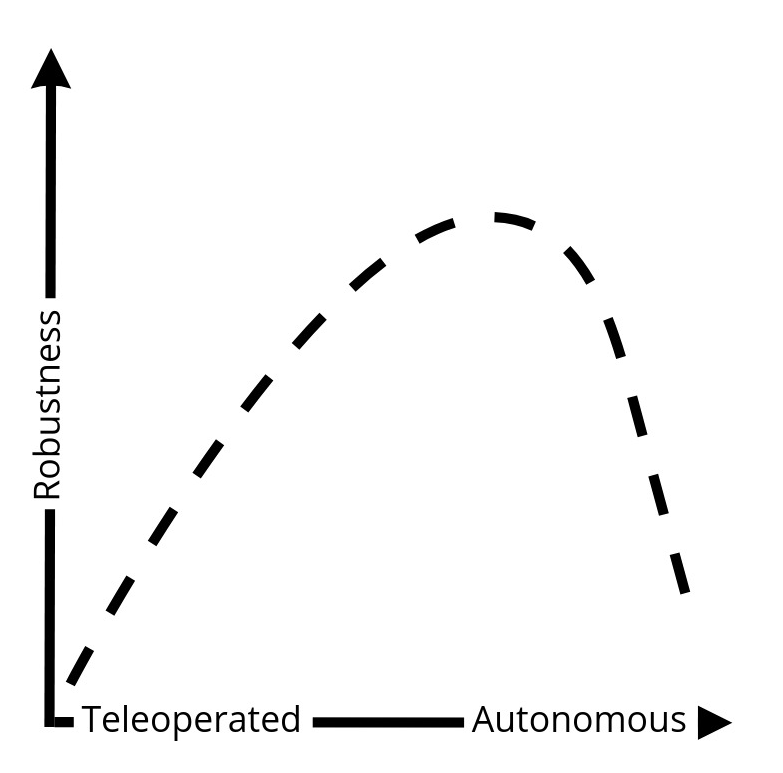
\includegraphics[width=0.285\textwidth]{img/autonomy_robustness.png}
    \caption{\textsc{Maximum Robustness is Achieved Through a Compromise}}
    \label{fig:autonomy_robustness}
\end{figure}
\noindent
It is obvious, but also important, that in a dynamic environment it is not possible to anticipate every possible type of failure and respond with appropriate recovery.
\cite{Meeussen:2011} For Meeussen et al., this is another motivation for including a human operator as a fallback solution. Their key insight for this thesis is the importance of having
a human \textquote{in-the-loop} to achieve robust long-term autonomy, where the robot acts autonomously most of the time but has the option to request help from a human operator
when needed. They strongly suggest that this type of semi-supervised control, with a focus on fault detection and recovery, has the potential to realize systems that actually deliver
practical benefits.\newline
Dayoub et al. \cite{Dayoub:2011} intend to equip long-term autonomous mobile robots with the ability to localize in changing environments. It is an early work on long-term mapping,
i.e., updating environmental knowledge over time, which, unlike static representations, takes into account the inherent dynamics of the real world. The authors facilitate the concepts
of long-term and short-term memory as well as hybrid metric-topological maps.\newline
In \cite{Veloso:2012}, Veloso et al. present their autonomous mobile service robots for indoor applications, which they call \textit{CoBots} (2012). Of particular interest to this thesis
is their focus on symbiotic autonomy, through which the authors allow the \textit{CoBots} to overcome their specific limitations by requesting help from humans.
Additionally, they propose to investigate robust execution monitoring strategies.\newline
Tipaldi et al. \cite{Tipaldi:2013} introduce a probabilistic localization framework for long-term autonomous systems, particularly acknowledging environment changes during
long-term operations. They state that previous approaches to localization in dynamic environments often treated dynamic objects as outliers and that this is insufficient
for semi-static objects that are naturally part of such environments.\newline
It should be noted that there is not a great deal of research providing actual long-term experiments with autonomous robots, mainly for two reasons:
Long-term studies are obviously more time-consuming and tedious, especially in real-world outdoor environments, and furthermore it is only in recent years that it has become
reasonably realistic to conduct such experiments based on technological progress. \cite{Leite:2013}\newline
In a special issue on long-term autonomy (2013), Barfoot et al. \cite{Barfoot:2013} ask what challenges need to be solved to bring long-term autonomous robots into the real-world. They are concerned with
two main subjects: Localization and mapping in dynamic environments and lifelong learning. The general theme under which one could summarize this special issue is the idea that it is
not possible to know every relevant aspect of the world in advance - these robots must have learning capabilities.
In accordance with this, Mühlfellner et al. \cite{Muehlfellner:2015} present an approach for lifelong visual localization and mapping based on three steps:
\begin{enumerate}
    \item Offline map generation based on multiple recordings (incorporating environment dynamics)
    \item Selection of landmarks that are considered useful for localization
    \item Online localization
\end{enumerate}
The authors have an interesting facet to their approach: \textquote{\textit{[...] we are concerned not so much with maintaining an accurate model of the world, but rather with
maintaining a useful model.}} \cite{Muehlfellner:2015}\newline
In 2016, Biswas et al. \cite{Biswas:2016} discuss results and insights from deploying a team of mobile service robots (\textit{CoBots}) in dynamic, unstructured real-world office environments
for extended periods of time. They emphasize the need for execution monitoring, which they incorporate in the form of scripts that monitor the progress of tasks and relay help
requests to human operators as needed. A particular focus of the work is on the robustness of the systems and understanding the nature of faults through extensive logging.
Ultimately, they require the intervention of human operators only in very rare situations and provide stable, long-term autonomous operation in the office environments considered.
\newline
Of course, there are not only long-term autonomous ground vehicles (AGVs). There is perhaps even more literature regarding the application of autonomous underwater vehicles (AUVs)
(e.g. \cite{Jones:2012}, \cite{Spears:2014}, \cite{Kunz:2009}, \cite{Chrpa:2015}, \cite{Harris:2021}) and unmanned aerial vehicles (UAVs) (e.g. \cite{Brommer:2018}, \cite{Dong:2014},
\cite{Dong:2017}) for extended periods of time. AUVs are particularly used for scientific observations and security applications. \cite{Chrpa:2015}
Steinberg et al. \cite{Steinberg:2016} debate challenges and opportunities for long-term autonomous systems in
maritime applications. They argue that many of the previous attempts in the literature targeting autonomous systems fail when the environment varies during deployment, e.g.,
due to weather or seasonal effects. The work identifies three main types of challenges for long-term autonomous systems:
\begin{enumerate}
    \item Transience of initial knowledge of state, environment, goals, etc.
    \item Insufficiencies of traditional fault monitoring / diagnosis due to extended operating times
    \item Demand for context-based constraints, priorities and goals
\end{enumerate}
The authors highlight that most autonomous maritime operations in the literature are of short duration and that humans must intervene whenever an unexpected situation arises. 
Furthermore, the work underlines the demand for robust solutions even when the environment and context changes heavily. What will also be of particular importance
in this thesis is their view of the human operator. They do not envision autonomous systems that should completely abandon human cooperation, but point to the importance of
appropriate communication channels (dialogue / explanations) for autonomous systems.\newline
One approach to long-term autonomous navigation is vision-based route following, which enables robotic systems to autonomously follow routes that were previously demonstrated
manually. \cite{Paton:2016} However, as the authors claim, to be able to use such approaches in actual long-term scenarios, the algorithms must be able to address the challenge
of extreme appearance changes in dynamic outdoor environments. The work presents a route following algorithm for autonomous systems that addresses the problem of changing appearance
by facilitating multiple channels of information, allowing to extend the autonomous capabilities to longer time periods. Yet, the paper claims that this approach is insufficient for
true long-term autonomy that covers seasonal changes and point to the promising field of multi-experience localization.\newline
Palomeras et al. \cite{Palomeras:2016} are investigating robust long-term autonomous underwater vehicles in real-world environments with a focus on minimizing human surveillance.
The authors point out that this requires methods for error detection and correction. The work is mainly focused on developing a framework that integrates many aspects previously
demonstrated into a holistic and robust solution. They are able to demonstrate a reasonably functioning system, but also hint that future work will need to enhance robustness to
unexpected failures, e.g., by incorporating redundancy.\newline
One of the most influential projects in the field of long-term autonomous robotics is the \textit{STRANDS} \cite{Hawes:2017} project (2017). The goal of the project is to integrate all the
artificial intelligence and robotics technologies necessary to create a long-term autonomous mobile service robot in a care facility environment. Thus, it is again an example for a project
that focuses on indoor environments. Special emphasis is placed on the application of the systems in real everyday environments as opposed to specific laboratory installations.
Furthermore, the robots are supposed to improve their behavior during their long-term missions by learning the dynamics of their environment, thereby increasing their robustness.
For the authors, the attribute \textquote{long-term} implies that the robot should be able to run continuously and autonomously in its environment for at least several weeks, which requires
a certain resilience.
An example of a study that emerged from the \textit{STRANDS} project is a study of autonomous service robots deployed in a nursing home by Hanheide et al. \cite{Hanheide:2017}.
Although the work concentrates on aspects of human-robot interaction, it is a relevant example of long-term autonomous use of a mobile robot in a real-world environment.
Their robot was in fully autonomous operation for $63$ days.\newline
Santos et al. \cite{Santos:2017} focus on spatio-temporal environment representations during long-term autonomous operations of mobile robots with the goal of constantly updating
and refining the robot's knowledge of its dynamic environment during the application. They view it as a never-ending task of acknowledging environmental changes, which is a key
requirement for long-term autonomy without human intervention. \cite{Santos:2017}
Another method for long-term spatio-temporal mapping in a mobile robot scenario in dynamic environments is presented by Krajnik et al. \cite{Krajnik:2017}. Their work is also
based on the assumption that environmental changes are usually subject to certain periodicities and routines. They are able to represent dynamics and predict future conditions
in the robot's environment.\newline
Schuster et al. \cite{Schuster:2017} introduce the \textit{Lightweight Rover Unit (LRU)} and study autonomous planetary exploration with its specific hurdles, such as
inherent communication delays. Due to these delays, teleoperation is generally infeasible for planetary rover applications, and a certain level of autonomy is mandatory for successful
operation. \cite{Schuster:2017} Leaving aside all the aspects that are crucial for missions on other celestial bodies but less relevant to the scenario of this thesis, there are
still a number of useful insights. For instance, their view of robustness based on local recovery. Whenever a malfunction occurs due to certain environmental conditions, this should
be recognized and dealt with locally. \cite{Schuster:2017} The authors propose defining fallback strategies for such cases, such as retrying the procedure in the simplest case. Even
under the severely limited communications with planetary rovers, the authors emphasize the need for external (ground station) monitoring and intervention capabilities, which they
consider obligatory for any system operating in an unknown environment. Thus, they rely on shared-autonomy whenever necessary. The work describes various recovery methods for failure
cases, such as scripts that can be used to reinitialize failed hardware components or to adjust parameters. Another crucial aspect for increasing robustness is seen by the authors
in redundancy, which seems reasonable in light of the limited response options due to the communication delay.\newline
Del Duchetto et al. \cite{DelDuchetto:2018} address navigation failures in long-term autonomous mobile robot applications with a human-in-the-loop learning approach that provides
recovery policies. The approach is based on the \textit{learning by demonstration} paradigm that facilitates human demonstrations to learn failure situations and appropriate recoveries.
Whenever a robot is confronted with a situation for which it has no recovery strategy, it requests a new demonstration. As many before, the work deals with long-term service robots to be used
in indoor environments populated by humans, specifically in nursing homes. The authors fundamentally share the global goal of this thesis and focus on one specific aspect, namely the
detection and correction of navigation failures, but they also emphasize the need for a general framework for error detection and resolution for long-term autonomy.\newline
Han et al. \cite{Han:2018} work on a sub-field of long-term autonomy that has received a lot of attention in recent years - long-term place recognition. This is an important aspect
of long-term autonomous systems, particularly in outdoor scenarios. Outdoor environments over extended periods of time are naturally subject to significant change (day time,
seasons, etc.). \cite{Han:2018} Their method for long-term autonomous place recognition \textit{HALGE (Holism-And-Landmark Graph Embedding)} represents places by using both semantic
landmarks and holistic scene information. The idea of long-term location recognition is to be able to detect whether the place where a robot is currently located is a
previously visited place and, if necessary, to identify it in the history (loop closure). \cite{Han:2018} Long-term place recognition is an essential milestone on the way to robust
localization and thus long-term autonomy of mobile robots in general.\newline
In 2018, Brommer et al. \cite{Brommer:2018} study long-term autonomy of unmanned aerial vehicles, which are also commonly used for monitoring purposes in precision agriculture. One problem with using such
systems in long-term scenarios is their limited battery capacity, which allows only relatively short deployments, e.g., of $15$ minutes. \cite{Brommer:2018}
To address this drawback, the authors develop an autonomous landing and recharging procedure. Since GPS is not necessarily accurate enough, the authors use a visual approach to
landing. They also introduce a state monitoring system that keeps track of critical aspects such as unexpected low battery and triggers a response when needed.\newline
A further very relevant work is written by Kunze et al. \cite{KunzeSI:2018}, who discuss challenges for long-term autonomous robots in real-world environments and how these can be addressed with techniques from the field of AI.
First, they note that such systems must be both hardware and software robust, meaning that the systems must be able to cope with any potential environmental changes expected
during their deployments. \cite{KunzeSI:2018} They point out that much of the long-term autonomy research focuses on coping with changing environments. The work suggests that
long-term operation could be an opportunity to improve the robustness and overall performance of the robot over time, e.g., through log analysis and manual improvements or machine
learning approaches. The key message of the special issue is that there are numerous applications and opportunities for using AI methods to achieve or improve long-term autonomy,
or in other words, for combined research of AI and long-term autonomy.\newline
A recent example of long-term autonomous tour guide robots is provided by Wang et al. \cite{Wang:2018}. They state that autonomous robots deployed over a long period of time are
particularly prone to failure, as the duration of the deployment introduces more uncertainties and corner cases that rarely occur in short-term applications. Based on their deployed
robots \textit{TritonBot} and \textit{BoxBot}, they are able to closely investigate problems in terms of long-term autonomy and resilience. In particular, they draw attention to
certain hardware and software failures, infeasible workflows, and human-robot interaction problems. The authors underline that certain errors are inevitable and that it is therefore
crucial to equip the robot with failure detection and fail-safe capabilities to achieve a certain level of reliability. Furthermore, they claim that it may be useful to establish a form
of component-level monitoring, which is fairly consistent with the approaches described in section \ref{sec:sim_and_mon_of_lta_challenges}. Another important aspect the authors
stress is that certain failures, especially hardware failures, occur so infrequently that they often go unnoticed. However, since they will occur in long-term autonomous operation,
it is essential to find a way to systematically and reproducibly evaluate potential failure cases, e.g., through simulations. \cite{Wang:2018} This is precisely the rationale behind
all the simulations described in section \ref{sec:sim_and_mon_of_lta_challenges}. The paper also suggests that it is advisable to design the software components in such a way that
they tolerate the temporary unavailability of other components and wait until the recovery is completed. Finally, as a further important remark for this thesis, they note that
comprehensive logging in long-term autonomous applications offers great potential for evaluation, testing, and learning, e.g., through the use of the ROS tool \code{rosbag}\footnote{Tool to record and play back data on ROS topics (\textcolor{link-color}{\url{https://wiki.ros.org/rosbag}})}.\newline
Egerstedt et al. \cite{Egerstedt:2018} consider a long-term autonomous environment monitoring scenario in which they define survival constraints inspired by the bond between
biological organisms and their environment in ecology. First, the authors highlight the unique challenges of long-term deployment in a dynamic, unstructured environment, such as
agriculture, noting that robots must have adaptive capabilities and manage problems potentially affecting their survivability. \textquote{\textit{The basic issue of survivability
over long time periods remains an open problem for autonomous robotic systems in uncontrolled environments.}} \cite{Egerstedt:2018} The work claims that survivability has been
previously addressed either by planned tasks that enforce survivability, such as battery station revisits in the scenario described in section \ref{sec:lta_plant_observation},
or by defining specific survivability goals that are combined with other objectives, i.e., multi-objective optimization. However, the authors point out that survivability is a
necessary condition for any successful operation and therefore a constraint-based approach may be preferable, based on the idea of ensuring survivability during the optimization
of an objective function. A very important aspect of long-term autonomous applications highlighted in the paper is that \textquote{\textit{[...] any assumption about environmental
stationarity, or even predictability, are doomed to be incorrect}}. \cite{Egerstedt:2018} They conclude that drastic environmental changes can lead to infeasible assumptions and
dysfunctional controls. Thus, they prefer to rely on low-level constraints that ensure safety and robustness and assume nothing about the environment.\newline
An important overview of the state of the art in artificial intelligence for long-term autonomy has been provided by Kunze et al. \cite{Kunze:2018}. The authors point out that there
are still many challenges to be overcome with respect to the reliable deployment of long-term autonomous robots in dynamic, partially unknown real-world environments. As essential
AI building blocks, they identify \textit{navigation \& mapping}, \textit{perception}, \textit{knowledge representation \& reasoning}, \textit{planning}, \textit{interaction}, and
\textit{learning}. All of these aspects have been major research areas in the AI / robotics literature for decades. The survey emphasizes the importance of bringing all of these
facets together to actually create systems that work in a practical way. Particularly relevant to this work are the identified natural challenge of system integration, i.e.,
integrating numerous methods and technologies into a comprehensive solution for long-term autonomy, as well as the design of ``human-in-the-loop'' systems capable of utilizing the
help of human operators in unexpected problematic situations. \cite{Kunze:2018}\newline
A very recent example of a long-term autonomous mobile robot serving as a tour guide in a museum is provided by Del Duchetto et al. \cite{Duchetto:2019}, who present their robot
\textit{Lindsey} (2019), which is designed to have better social abilities compared to previous models. However, since the focus of this thesis is not on human-robot interaction, another aspect of the work is of
greater relevance - their approaches to dealing with contingencies. A useful monitoring interface that can be used to observe and, to a limited extent, control the robot via a web
application is developed. They note that it is obligatory for long-term autonomous robots that operate without the supervision of a human operator to be able to communicate
problems and situations that the robot cannot handle itself. In the work, a ROS module is developed in which operators can specify problematic conditions that are then constantly
checked during runtime. As soon as such a condition occurs, the information is transmitted via a specific channel. This allows the operator to respond to faults without having to
permanently monitor the robot's activities. Human-robot communication in this thesis operates in an analogous manner (cf. section \ref{sec:fallback_solution}).\newline
Tomy et al. \cite{Tomy:2019} study a specific aspect of long-term autonomous mobile robots, namely their charge scheduling. It is emphasized that the actual operating times of
such systems are mainly determined by their battery capacities and that most systems simply use certain thresholds to determine charging stops. With the work, the authors attempt
to improve this by relying on the fact that long-term autonomous robots have ample opportunity to learn adequate charging times and match them to natural idle times, etc.\newline
Krajnik et al. \cite{Krajnik:2019} and Fentanes et al. \cite{Fentanes:2015} propose methods for modeling and dealing with variations in the environment in long-term mobile robotic
applications caused by human activities or natural processes, based on the assumption that such events are often periodic and not entirely random. They claim that the long-term
nature of such operations is not only a challenge but also a chance to learn how the environment changes and to identify certain regularities. They further note that this ability
allows the robot to predict the future state of the world based on the recognized patterns, which certainly has a positive impact on long-term autonomy performance.\newline
With manipulation under uncertainity, Lanighan et al. \cite{Lanighan:2019} work on another aspect of long-term autonomous robotics. They consider a robotic system with a monitoring and
cleaning task in a dynamic environment where it is expected to operate autonomously for extended periods of time without human supervision. They see the uncertainty in unstructured
dynamic environments as the greatest challenge to long-term autonomy and highlight the need for planning and execution approaches capable of dealing with such uncertainties and
inherent risks. They model the problem as a \textit{Partially Observable Markov Decision Process (POMDP)}, plan in the belief space, and try to avoid unrecoverable situations by
managing the stochastic actions.\newline
Recently (2020), Basich et al. \cite{Basich:2020} introduced a method for robots to improve their competence during long-term autonomous applications. Their particular focus is on so-called
\textit{competence-aware systems}, which are able to rate their own feasible level of autonomy under certain circumstances. This competence must be learned through feedback
(reinforcement learning) from human operators. The idea is that over time, the level of autonomy increases and the dependence on the human operator diminishes as the robot creates
finer models of its environment.\newline
Also just recently, Kyberd et al. \cite{Kyberd:2021} presented their work on long-term autonomy in diverse outdoor environments. They emphasize that the focus in the literature to date
has been on indoor environments due to hazardous weather conditions and the like in outdoor settings. The work introduces design principles for unmanned ground vehicles suited to the specific
intricacies of operating outdoors, with special emphasis on redundant safety layers and the ability to function in harsh weather and lighting conditions. Since their systems
lacks an autonomous charging procedure, a human operator is notified whenever the robot needs to be recharged. The authors indicate that in the future they will aim for autonomous
charging, e.g., by inductive charging, so that the entire operating cycle can be captured autonomously. This is exactly what the integration of autonomous docking described in section
\ref{sec:docking_solution} aims to achieve in this work.\newline
Eventually, in 2021, Emam et al. \cite{Emam:2021} present a \textit{Control Barrier Function (CBF)} framework to tackle the problem of perturbations that the robot may face. The authors
underscore that when developing new algorithms for robots operating autonomously for extended periods of time in dynamic environments, it is imperative to pay close attention to
robustness in order to deal with all the challenges potentially occurring in such situations (cf. section \ref{sec:challenges_for_lta}). As they claim:
\textquote{\textit{[...] if these disturbances are not addressed, the possibility of failure becomes almost assured if the robots are required to operate over long time horizons.}}
\cite{Emam:2021} Accordingly, the work indicates the need for robust control mechanisms capable of dealing with such contingencies.\newline

\noindent
\textit{Execution Monitoring}\newline

\noindent
An early work on execution monitoring in robotics is by Pettersson \cite{Pettersson:2005} (2005). The author attempts to transfer the knowledge of \textit{fault detection and isolation
} (FDI) commonly used in industrial control to the field of robotics. The work already highlights the requirement for execution monitoring when planning the deployment of robots in
dynamic environments, e.g., due to lack of information, unreliable resources, or stochastic effects. Pettersson discusses several attempts to deal with uncertainty, but notes that
there is no way to completely eliminate uncertainty in partially observable dynamic environments and that systems must tolerate some degree of uncertainty. The paper asserts that
systems must expect faulty execution from time to time, e.g., by including execution monitoring as part of the control architecture. This is exactly what is done in this thesis
(cf. section \ref{sec:execution_monitoring_smach_architecture}). Pettersson compares several definitions for execution monitoring. A classic variant from the field of AI is the
identification and classification of inconsistencies between observations and predictions, and mechanisms to recover from these inconsistencies. \cite{Pettersson:2005}
However, according to this definition, only systems with predictive models can perform monitoring. \cite{Pettersson:2005} A second definition, which comes more from an
industrial control perspective, defines it as a continuous process of real-time information acquisition that determines the state of the system and signals anomalies.
\cite{Pettersson:2005} Based on the literature, Pettersson proposes three types of general functions of a monitoring procedure, the first two of which are more or less mandatory:
\begin{enumerate}
    \item Fault detection \textrightarrow $\thinspace$ recognizing problem
    \item Fault isolation \textrightarrow $\thinspace$ classifying error type
    \item Fault identification \textrightarrow $\thinspace$ rating severity
\end{enumerate}
Following the definitions in the paper, the execution monitoring procedures described in section \ref{sec:sim_and_mon_of_lta_challenges} fall under the category of data-driven
approaches, where fault detection and isolation are based on the (statistical) evaluation of the input data. Statistical analysis assumes that data variability changes drastically
only in problematic situations and is otherwise relatively stable. \cite{Pettersson:2005} Many of the monitoring methods presented in this thesis involve comparing an input signal
to a specified limit (cf. section \ref{sec:sim_and_mon_of_lta_challenges}), which is called \textit{limit value checking} and is very common in industrial control. \cite{Pettersson:2005} However, the methods in this thesis are also
quite well aligned with the core ideas of expert systems (knowledge-based systems), which often represent knowledge with conditional statements. \cite{Pettersson:2005} Pettersson,
like many other authors, points out that one of the most common problems in the field of mobile robotics is that methods and solutions are developed and tailored for a specific
system and the generalizability is rather limited, which is a motivation for developing solutions that are as general as possible but still useful.\newline
In 2014, Vechet et al. \cite{Vechet:2015} state that fault detection is underexposed in robotics research and development, but is nonetheless fundamental to the
deployment of autonomous mobile robots. They see a demand for health monitoring to prevent system failures and present a Markov chain model for FDI.\newline
Iocchi et al. \cite{Iocchi:2016} develop a framework for plan generation and execution with a focus on robustness by addressing certain shortcomings of classical plan execution
monitoring approaches. They are evaluating the framework in a service robot application in public, human-populated environments such as shopping malls and offices. A critical
challenge in such an environment, identified in the paper, arises from the fact that the robot must interact with inexperienced users. In particular, they highlight the great
significance and need for planning under uncertainty, execution monitoring solutions, and the combined consideration of planning and execution when it comes to the use of
autonomous robots in real-world environments populated by humans. The framework proposed in the work relies on \textit{Progressive Reasoning Units} and \textit{Petri Net Plans}
and is, like many works in the literature considering monitoring, particularly focused on plan execution.\newline
In 2016, Winder \cite{Winder:2016} proposes an anomaly reasoning framework capable of recognizing and responding to previously unknown entities and situations, with the overall goal of
increasing an agent's versatility and robustness in dynamic environments. The author postulates the hypothesis that such an approach requires the integration of machine learning
methods and systematic knowledge representation.\newline
Khalastchi et al. (2018) consider \textit{fault detection and diagnosis} (FDD) for robotic systems, which is necessary for recovery from problematic situations and thus
robust long-term operation. \cite{Khalastchi:2018} The application of FDD to robotics is a relatively new field of research, but one that is very crucial
because errors can disrupt a robot's mission, reduce its efficiency, or even pose safety problems for itself or the environment. \cite{Khalastchi:2018} The paper notes that it is
critical that the detection of a problem is followed by some form of diagnosis that identifies the affected component and supports the recovery process. The authors provide a useful
fault taxonomy for robotic systems in which they generally divide hardware (detection, action), software (algorithms, implementations), and interaction (internal / external) faults.
Knowledge-based FDD methods, e.g., expert systems such as the ones proposed in section \ref{sec:sim_and_mon_of_lta_challenges}, are essentially based on predefined issues and
diagnoses. \cite{Khalastchi:2018} The authors note that internal sensors that provide information about the current state of the robot can be facilitated in FDD. In addition,
exteroceptive sensors should be used for this purpose, but of course they can be used not only for FDD, but also can be the target of FDD in case of sensor failures. \cite{Khalastchi:2018}
As a major challenge, the authors see the real-time nature of robotic applications, where erroneous situations must be detected as quickly as possible so that the robot can resume
its operation. Usually, FDD must be performed on board the mobile robot, which imposes significant constraints on computational resources. \cite{Khalastchi:2018} As mentioned earlier,
the monitoring approaches in this thesis are model-free, which has the advantage of providing some generality and thus transferability to other systems and scenarios. \cite{Khalastchi:2018} 
In addition, the authors emphasize that trying to model every aspect of the system as well as its interaction with the environment is very complex and often infeasible.
However, they also illustrate the disadvantage of expert system approaches, namely dealing with the unknown, since it is not trivial to extrapolate from a fixed ruleset.\newline
A somewhat different perspective is provided by Honig et al. \cite{Honig:2018}, who review methods for fault detection and recovery with a particular focus on human-robot interaction. Nevertheless, the work contains several aspects
that are quite relevant for this thesis, despite their different focus. First, like many authors before, they emphasize that robots working in dynamic real-world environments are
constantly confronted with errors and that there is still a lack of proper error management methods. Consistent with the literature, they define a \textit{failure} loosely as a
state in which the performance provided by the robot deviates from the norm, caused by one or more \textit{errors}, which they consider system conditions that lead to such
situations. Additionally, they consider \textit{errors} as the result of \textit{faults}, which are ultimately the reason why the system gets into such an error state.
The authors discuss numerous taxonomies for classifying failures and compare various concepts from the literature. Of particular
interest to this work is the concept of terminal failures that break the current mission of the robot, non-terminal failures that merely affect the outcomes or performance and
reparability of such cases. Also useful is their discussion of failure categories, which largely coincide with the categories of Khalastchi et al. (interaction, hardware, software).
\cite{Khalastchi:2018}. The authors themselves focus on the distinction between technical failures (hardware / software) and interaction failures (environment / other actors).
Of crucial importance to this work is the authors' finding that the involvement of a human operator in certain critical situations is computationally cheaper than comparatively
costly and often unreliable other approaches. To do this in the most effective way, the problem should be communicated as precisely as possible. \cite{Honig:2018}\newline
In 2019, Mauro et al. \cite{Mauro:2019} introduce a high-level deep learning and vision-based approach to execution monitoring for robot tasks. Monitoring is again limited to the execution of the
plan and not to the operation of the robot in an environment in general. They evaluate their approach with a humanoid assistant robot in a warehouse environment and report some
promising results. However, as mentioned, it is only considering very specific tasks and high-level actions.\newline
Recently (2021), Harris et al. \cite{Harris:2021} presented an execution monitoring and online plan modification approach that considers aspects such as resource availability
and goal reasoning. The approach is evaluated in a long-term AUV scenario with very limited opportunities for human intervention and a highly dynamic and uncertain environment.
Their method is based on the idea of altering the plan as needed, e.g., adding goals when the resource consumption is lower than expected and removing goals (starting with those with
low priority) when it is higher than expected. In order not to generate infeasible plans, the method relies on information about the causal relationship between actions. In cases
where resources are uncertain, one approach is to provide branches in plans that allow a decision to be made between multiple options based on available resources. \cite{Harris:2021}
The general monitoring and resolution approaches developed in this thesis are not as tethered to a plan, but the overall ideas and goals are similar.\newline
Not necessarily focused on execution monitoring, but a good motivation for its necessity is provided by \cite{Roucek:2021}, which asserts that research papers are
usually concerned with aspects such as accuracy or computational complexity of their methods, but not so much with their reliability in integrated systems such as robots.
And further: \textquote{\textit{[...] the performance of robotic systems cannot be optimal in real-world situations which are impacted by the robustness of the deployed systems}}.
\cite{Roucek:2021} They conclude that the successful deployment of robots in real-world environments fundamentally depends on reliability and interoperability aspects of the
employed submodules, which is a great motivation for this thesis.\newline
Very recently, Coruhlu et al. \cite{Coruhlu:2021} studied plan execution monitoring for autonomous systems. They point out that it is critical to equip robots with the ability
to recognize and respond appropriately to deviations between expectations and observations, focusing particularly on diagnosis and explanation. Although at first glance their work
appears to be very closely related to this thesis, their focus is quite different in that they are concerned with high-level monitoring of plan execution, dealing in particular with
partial observability. As with most execution monitoring work in the literature, the focus is on plan execution rather than general robot operation in an environment, recovery often
relies on replanning.\newline

\noindent
\textit{Environment Monitoring and Agricultural Robotics}\newline

\noindent
An early example of automated crop monitoring in its broadest sense is forest inventory. In 2006, Lalonde et al. \cite{Lalonde:2006} address the task of automatic and accurate tree counting and
diameter estimation based on $3D$ point cloud processing. The motivation in this area is similar to the classic field scenarios: Optimizing efficiency and reducing manual labor.\newline
Singh et al. \cite{Singh:2010} (2010) present their results and findings from operating a reconfigurable autonomous driving system on a farm. Their overall goal is to integrate technologies
from the field of robotics with plant science to increase production efficiency. Based on the reconfigurable tool and sensor setup, they aim to use the systems to improve the
efficiency of various agricultural operations such as harvesting, spraying, plant inspection, tree counting, etc. The vehicle drives autonomously in the sense that it detects and
follows rows of trees in an orchard based on laser scans. One of the most important insights, which may also be relevant to this work, is that it is crucial to keep the project
consistent with the actual requirements of the intended users and real-world applications. Only then can the result actually be of use to practitioners.\newline
Xue et al. \cite{Xue:2010} present a vision-based system also capable of guiding a mobile robotic platform through crop rows in a field, thus enabling autonomous navigation
in a field. The work stresses the need for reconfigurable platforms that can, in principle, be used for various agricultural tasks, depending on the particular sensor equipment.
\newline
A comprehensive overview of robotic systems (AUVs, AGVs, UAVs) for environmental monitoring, e.g., deep-sea or volcano exploration, is provided by Dunbabin et al. \cite{Dunbabin:2012} in 2012.
The authors underscore the urgent need for long-term autonomous environmental monitoring systems to cope with natural catastrophes such as earthquakes, tsunamis, forest fires, volcanic
eruptions, etc. In a nutshell: \textquote{\textit{[...] scientists see robotics as a promising tool with the capacity to improve their current means to observe and collect
data about natural processes or phenomena at vast spatial and temporal scales.}} \cite{Dunbabin:2012} They view robots essentially as mobile sensors that are used to understand
the environment. Although there is an undeniable demand for such systems, the authors note that there is a lack of robustness, reliability, and security for a widespread use,
which could be addressed by fault-tolerant systems and redundant hardware components. \cite{Dunbabin:2012}\newline
In 2014, Dong et al. \cite{Dong:2014} present an imaging method for crop monitoring based on both AGVs and UAVs. Traditionally, manual labor has been required to collect samples, which is
obviously not suitable for monitoring large areas over long periods of time. \cite{Dong:2014} Therefore, as the authors point out, imaging methods have been developed to enable
remote sensing and reduce the human effort required for data acquisition. Originally, hyper-spectral satellite imagery was used with the disadvantage of limited spatial and temporal
resolution. \cite{Dong:2014} Thus, they introduce a crop monitoring approach that uses UAVs or AGVs and methods from computer vision to increase the efficiency of crop imaging.
The goal of the work is to create a $4D$ representation of plant development based on high-resolution imagery and GPS / IMU data. The overall goal of the work is to increase the
efficiency of agricultural production by replacing time-consuming and costly human labor with highly efficient autonomous monitoring systems.
As an early work, however, it is still limited to manually operated vehicles and therefore disregards the aspect of autonomy in this sense.\newline
Bargoti et al. \cite{Bargoti:2015} introduce a system for automated tree detection on an apple orchard that combines image data and laser scans. The work highlights that information
acquisition and processing is becoming increasingly relevant for farmers trying to optimize the efficiency of their processes. The developed system is a UGV capable of autonomous
operation via intrarow navigation. However, the authors point out issues regarding localization reliability and GPS connectivity that need to be addressed in future work.
This is a strong motivation for two of the challenges discussed in section \ref{sec:challenges_for_lta}.\newline
In 2015, Carlone et al. \cite{Carlone:2015} highlight that recent advances in mobile robotics, particularly UGVs and UAVs, are increasingly providing a realistic alternative to
inefficient, labor-intensive manual work in the task of continuous crop monitoring. They target a specific aspect of crop monitoring and create $3D$ representations over time,
resulting in an overall $4D$ model of plant evolution. \newline
Virlet et al. \cite{Virlet:2016} choose a completely different approach of automating plant phenotyping. They are developing an automated field phenotyping platform, but instead of
relying on (autonomous) vehicles, they are building a sensor array mounted on stationary rails above the rows of plants to be monitored. They argue that such a system has the
advantage of completely eliminating the need for human supervision, which is not yet the case with vehicles. A further disadvantage of vehicle-based monitoring systems is their
impact on the soil structure and its potential damage, especially because of the continuous nature of the operations. \cite{Virlet:2016} Thus, they provide an interesting
alternative to autonomous monitoring using AGVs, which arguably has a higher initial effort to set up such a monitoring structure, but may be more reliable and soil-protecting,
at least with the current state of the art of AGVs. However, one could argue that such an approach may not scale for very large field areas.\newline 
Another semi-autonomous mobile ground vehicle for crop monitoring is presented by Bietresato et al. \cite{Bietresato:2016}.\newline
In 2016, Bechar et al. \cite{Bechar:2016} provide an overview of the current state of the art of agricultural robots for field work. The authors particularly emphasize that the various
components that make up a robotic system must be integrated and synchronized to create a holistic system capable of performing in unstructured dynamic environments at least as
well and reliably as previously used methods, such as manual human labor. Successful systems that are rarely available on the market must be economically viable, safe and robust.
\cite{Bechar:2016} In specific, the authors stress the necessity of researching human-in-the-loop systems, as they see great potential in them for increased robustness and
reliability. The paper summarizes the extensive research that has demonstrated the potential of robots to address current and future problems in agriculture, particularly in terms
of production efficiency and environmental sustainability. As one of the biggest challenges in agricultural scenarios, they identify the unstructured and dynamic nature of the
environment, which changes over time and implies myriad unpredictable contingencies. Bechar et al. classify applications of robotic systems in general into four groups:
\begin{itemize}
    \item Environment and objects structured
    \item Environment unstructured and objects structured
    \item Environment structured and objects unstructured
    \item Environment and objects unstructured
\end{itemize}
They place the agricultural sector in the last and arguably most difficult category, which they see as a particular hurdle to commercialization. Based on their reasoning, it is
evident that the challenges to long-term autonomy that will be considered in this thesis are part of the barrier to commercialization. Another challenge identified in the work that
is particularly relevant to this thesis is that robotic systems and technologies developed for one specific agricultural use case are not necessarily reusable for others because they
are so different, i.e., it is difficult to find generic solutions. Nevertheless, it should be an important aspiration to develop solutions as generic as possible in terms of sensors
used, etc., which is taken to heart in this thesis. Regarding the autonomy of such systems, the authors believe that partially autonomous robots will undoubtedly be useful in
practice, even if they do not yet achieve full autonomy. The paper examines numerous research papers and concludes that there are very few commercially available solutions, all of
which are the result of iterative development for a very specific task. The authors note that the early examples of autonomous systems clearly suggest that the performance of the
system can be improved by human support in dynamically occurring problem situations, allowing some form of collaboration as human and robot capabilities tend to complement each
other. This is exactly the idea of this thesis, to cope with otherwise unsolvable situations. It is obvious that it is already a huge improvement when a robotic system can take over
a large part of the work and a human operator only needs to intervene once in a while in unpredictable and unsolvable situations. Full autonomy may be a reasonable goal to strive for
in the future, but it is not a requirement for improving productivity. The work also asserts that the most important aspect with respect to the numerous integrated components in a
robot is to provide methods capable of handling unexpected events, which is a great motivation for this work.\newline
In a later paper (2017), Dong et al. \cite{Dong:2017} revisit autonomous crop monitoring with a focus on high temporal as well as spatial resolution. They claim that common $3D$ models do
not acknowledge the temporal aspect of crops that are continuously growing and changing. As in the previous work, they rely on UAVs and AGVs because of their potential to collect
data at high spatial and temporal resolution very efficiently. They present a crop monitoring method for $4D$ representation considering both space and time, as well as an algorithm
for robust data association that can deal with heavy environment variations. The work assumes a static environment during a data acquisition process, which means that it ignores
unexpected dynamic changes that can be expected in real-world environments and focuses on the evaluation of the proposed methods. Moreover, the aspect of autonomy is still not taken
into account.\newline
Ampatzidis et al. \cite{Ampatzidis:2017} provide an overview of robotics and AI methods and technologies applied to the field of plant pathology as well as precision agriculture
in general. In addition to the advancing automation of classic agricultural processes, there is an ever increasing focus on automated detection of plant diseases.
\cite{Ampatzidis:2017} According to the authors, it is crucial that further research and development of sophisticated autonomous robotic platforms for agricultural purposes
goes hand in hand with the advancement of systems for diagnosis.
Many of the incorporated AI methods, such as those from the field of computer vision, are developed independently of
the robotic systems that use them in practice. \cite{Ampatzidis:2017} Thus, the authors highlight the need for integrated testing and diagnosis.
Likewise, \cite{Roucek:2021} underlines the fact that robots consist of a large number of integrated hardware and software modules that are typically developed and
tested in isolation, which is why aspects such as system integration, interoperability, etc. often unjustly receive little attention.\newline
In 2018, Roure et al. \cite{Roure:2018} study a monitoring and protection scenario in vineyards. Typically, human workers manually go through the field and distribute pheromone dispensers
to protect the plants. \cite{Roure:2018} The authors utilize a mobile AGV and focus on the necessary integration of state of the art robotics and AI techniques required to deploy
such a system.\newline
Very close to the scenario in this thesis in the work of Bayati et al. \cite{Bayati:2018}, which considers a mobile robot for crop monitoring. The authors present a high-throughput
plant phenotyping system for canola plants. Only such automated phenotyping systems are capable of efficiently providing the necessary information for plant breeding and related
genetic research. \cite{Bayati:2018} The authors claim that in 2018, there were no commercially available high-throughput plant phenotyping platforms (HTPPs) and especially no
autonomous vehicles. The goal of phenotyping is to identify desirable genetic responses to environmental stimuli in order to improve crop quality. \cite{Bayati:2018}
In the paper, a prototype of an automated HTP based on an agricultural vehicle is presented. However, it is not yet about full autonomy and especially not about long-term autonomy.
\newline
A recent work on real-time detection of crops for autonomous harvesting is provided by Montes et al. \cite{Montes:2020} in 2020. The work focuses on real-time detection of broccoli crops
in $3D$ point clouds.\newline
Also very recently, Fountas et al. \cite{Fountas:2020} gave an overview of the state of the art in robotic systems for agriculture, especially for field work. The authors distinguish
the challenges that such robots might face in general and task-specific issues. The universal issues are more related to challenges that all AGVs might face in dynamic outdoor
environments (terrain assessment, route planning, safety, etc.). \cite{Fountas:2020} Whereas task-specific issues are more related to the specific agricultural task. The authors
focus on problems specific to crop production, such as weed control, seeding, disease and insect detection, monitoring, phenotyping, spraying, and harvesting. Particularly relevant
to this thesis is the section on plant monitoring, where the authors underline the potential of automation in this area. There are systematic assessment tools such as
\textit{Ratio Vegetation Index (RVI)} and \textit{Normalized Difference Vegetation Index (NDVI)} that inform about important aspects of the overall plant health. \cite{Fountas:2020}
In general, the authors point out that robotics in agriculture has the potential to solve some of the fundamental efficiency problems that currently exist in the field. In summary,
they describe current research and commercialization efforts, highlight the technologies required for such systems, and hint to some potentials, particularly related to challenges
in computer vision that are ubiquitous in agricultural application of robots.\newline
In 2021, Polvara et al. \cite{Polvara:2021} consider a specific issue related to the increasing use of autonomous mobile robots in agricultural environments where they collaborate with
human workers. The authors present a method for identifying and tracking human workers in such environments to enable robots to become useful assistants.\newline
Finally, Khak Pour et al. \cite{KhakPour:2021} present an implementation of an autonomous, mobile, ground-based HTPP for crop monitoring. However, autonomy refers to the
monitoring task, but not to the entire operation, as the tractor is a semi-autonomous vehicle. Nevertheless, since the authors consider their system ready for the commercial
market in principle, it is a good example for the fact that full-autonomy is not necessarily the paradigm to strive for, at least not to be useful.\newline

\noindent
\textit{Concluding Remarks}\newline

\noindent
A substantial majority of the research described concerning long-term autonomy deals with indoor service scenarios. One could argue that this is a manual sample that may be biased,
however, it should fairly accurately reflect the focus in the literature. The examples available for outdoor scenarios tend to focus on very specific aspects of long-term autonomy,
such as environmental change and place recognition, which is briefly discussed in section \ref{sec:challenges_for_lta}. In addition, general problem handling capabilities are often
tightly tethered to specific systems and environments and therefore hardly reusable; sometimes they are not even explicitly described. What is perhaps a bit underexposed in the
literature is the big picture of long-term autonomous mobile robotic applications in outdoor scenarios, not focusing on specific aspects but approaching an integrated functioning
system. More precisely, work that discusses the common problems in all autonomous long-term scenarios, regardless of the specific application, and how to address them by merging
ideas from long-term autonomy and general execution monitoring. This thesis is intended as a step in the direction of thinking about a generic framework that is nevertheless specific
enough to be concretely applicable in the scenario under consideration. Referring to the overview of agricultural robotics, it should be emphasized that a fully autonomous mobile
robot is considered in this work. Most of the work in the literature considers autonomy in the sense that a system is able to autonomously follow plant rows, e.g., intrarow
navigation, but typically not a system that can freely and autonomously navigate through its environment. The work rarely considers full autonomy, and particularly not long-term
autonomy. As mentioned before, full autonomy is not necessarily the paradigm to strive for if the goal is to increase efficiency. If the tedious and dangerous tasks are taken over
by the robot and the human only has to intervene from time to time, it is a huge improvement, even if the human is still part of the work in a sense. Nonetheless, it is worth
investigating full autonomy for agricultural applications, whether or not it proves to be the best suited concept.

\vfill
\pagebreak

\section{Long-Term Autonomous Plant Observation}
\label{sec:lta_plant_observation}

The particular scenario that is going to be considered in this work takes place in an agricultural context. Therefore, the robot will be faced with a highly dynamic, unstructured
environment. Long-term autonomy in known, static environments is essentially solvable through robust systems that remain functional over extended periods of time. \cite{Kunze:2018}
Such environments are often given in an industrial context where robots must perform well-defined, repetitive tasks in a stable and predictable setting. \cite{Bechar:2016}
In contrast, a highly dynamic, partially unknown environment such as in this scenario poses much more difficult
challenges, e.g., due to unexpected environmental changes that are hard, if not impossible, to anticipate.
Such environments are often referred to in the literature as \textquote{automation-averse}.
The idea is to enable a mobile robot to autonomously conduct $3D$ lidar scans and hyperspectral images of the plants on a field in order to monitor their growth progression and 
to detect certain features based on the growth stage. Moreover, these recordings can be used to detect leaf diseases. It is essentially a task of data acquisition.
Correspondingly, the robot has to be able to process the entire field continually without the need for human supervision,
including the requirement for repeated charge stops. For this purpose, there is supporting infrastructure in the form of a container with an inductive charging station on site
establishing the power supply. Since the focus of the work is not going to be the scanning task, but to establish robust long-term autonomy, the actual detection of features 
etc. will be disregarded.\newline

\noindent
A crucial question is how to actually define ``long-term''. As Hawes et al. remark, it has no strict definition and can have various meanings depending
on the context, e.g., NASA's rover \textit{Opportunity} has been exploring the surface of Mars autonomously for years and autonomous wave gliders are able to monitor
ocean sections for months. Furthermore, there are mobile service robots used for extended periods of time in everyday, indoor environments like hospitals 
as examined in the \textit{STRANDS} project. \cite{Hawes:2017}
For this work, in contrast, ``long-term'' is going to be defined in terms of the robot's temporal radius of action that is mainly based on its battery capacity, i.e., charge cycle,
but may also include aspects like maintenance intervals etc. In general, all processes that require a number of such cycles are considered long-term processes.
Accordingly, ``long-term'' can only be defined depending on the system in question. To give an example: There are systems with very limited battery capacity, 
such as toy drones. Based on absolute time, a two-hour experiment might not be regarded as being long-term, but if it involves multiple charging cycles, it can be 
algorithmically considered a long-term process. Consequently, ``long-term'' is relative.\newline
In the agricultural sector, there are stages that last much longer than a charge cycle, e.g., vegetation periods.
However, the seasonal cycle is not the sort of long-term process that will be investigated in this work, as such processes already exist on a much smaller scale.
On the one hand, there is the mission level, i.e., one processing of an entire field.
Such a mission can already be regarded as long-term, since based on the dimensions of the particular field under consideration, it is not guaranteed that one
battery charge will be sufficient to cover the entire field. Instead, one battery cycle will be defined as sufficient to cover a certain fraction of the scan
positions, and a planner should maximize the number of planned scan stops in a mission under the constraint that a battery safety buffer is not undercut.
Thus, a key aspect of the scenario is going to be that the mission must be paused, the state must be saved, and the mission must be continued after recharging.
In the meantime, the environment may have changed, e.g., weather conditions or illumination, which is relevant for certain sensors of the robot.
On the other hand, there are going to be several such field processings during one vegetation period, which makes it a long-term process of repeated missions.
Hence, it takes a number of charge cycles to cover the entire field, and that mission is going to be repeated every few days,
which means that there are two different long-term cycles that are intertwined.
These two cycles basically represent a lower bound for the length of long-term autonomous episodes in the scenario under
consideration. Likewise, in contrast to the above examples of Mars rovers and autonomous wave gliders, which are long-term
processes of arbitrary length, it is useful to think about natural upper bounds on the length of such episodes in agricultural
applications. Such a natural upper bound could be a time after which a human operator will inspect the robot anyway,
which in agriculture is certainly the case sooner than after a few months, e.g., during maintenance sessions
when sensors such as cameras and laser scanners are cleaned, tire pressures are checked, etc.
After such a maintenance session, a new episode begins.
Based on these bounds, it makes sense that the robot does not send every minor problem it recognizes directly to the operator,
but keeps a list of minor issues that do not require immediate action, but should be resolved during the next maintenance
appointment.\newline

\noindent
Now that it has been sufficiently clarified how \textit{long-term} and \textit{mobile} are to be understood in the context of this work,
a precise definition of what is meant by the remaining attribute \textit{autonomous} follows.
Like the concept \textit{long-term}, \textit{autonomous} is not sharply defined in the literature and can have different meaningful connotations depending
on the context. Autonomy in the context of application-oriented robots usually has the goal of achieving a higher degree of automation in these applications,
i.e., using technical means so that a process runs completely or partially without involvement and supervision of a human operator. \cite{Hertzberg:2015}
Completely or partially already indicates that autonomy is not a binary attribute, but refers to a spectrum of different degrees of autonomy,
ranging from teleoperation at the lower end over shared and traded control up to full autonomy at the upper end. \cite{Hertzberg:2015}
Figure \ref{fig:autonomy_spectrum} summarizes these concepts based on \cite{Hertzberg:2015}.
\begin{figure}[H]
    \centering
    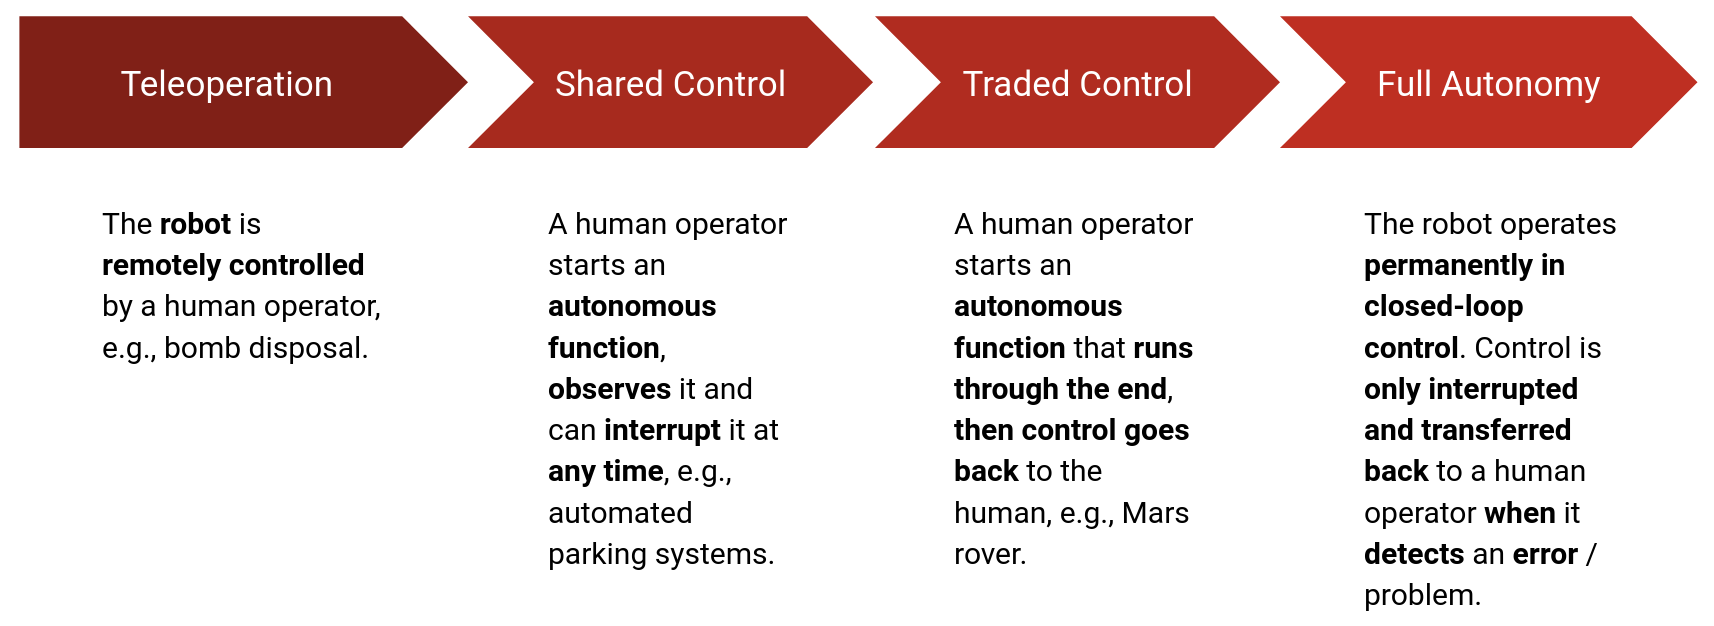
\includegraphics[width=\textwidth]{img/autonomy_spectrum.png}
    \caption{\textsc{Autonomy Spectrum}}
    \label{fig:autonomy_spectrum}
\end{figure}
\noindent
Accordingly, autonomy does not necessarily mean that there is no connection to a human operator at all.
The concept of traded control is particularly relevant for robotics in space applications, e.g., satellites or planetary rovers.
NASA's Mars exploration rovers \textit{Spirit} and \textit{Opportunity}, for example, do not operate fully autonomously, but rely on human assistance for many tasks,
such as plan generation and evaluation. \cite{Bresina:2005} NASA calls the concept \textit{mixed-initiative planning}. Involving humans in control has the advantage of gaining
flexibility, which allows to dynamically react to unexpected situations. \cite{Bresina:2005}
The idea is that the robotic system operates autonomously in principle, performing all the repetitive routine tasks, but the human operator can take over in certain situations,
such as when the robot is in danger and human intervention is required, or when a task needs to be performed that for some reason is better suited for a human operator.
\cite{Kortenkamp:2009} There is even evidence that \textit{human initiative} systems that can switch between different autonomy levels during operation perform better than
systems with fixed autonomy levels, at least in certain environments. \cite{Chiou:2021}
The plant monitoring robot considered in this work, however, can be classified as fully autonomous in the sense of figure \ref{fig:autonomy_spectrum}, 
i.e., during a long-term autonomous episode as defined above, the robot should only come into contact with a human operator when it detects an error or a problematic situation
that prevents it from continuing its task.

\section{Prototype Scenario in the Simulation}
\label{sec:prototype_scenario}

As starting point serves a physics simulation in \textit{Gazebo}\footnote{Open source $3D$ robotics simulator (\textcolor{link-color}{\url{https://gazebosim.org/}})} that has been created within the research project
\textit{PORTAL}\footnote{Plant breeding using robotics and AI for advanced data analysis and decision making in virtual spaces\\
(\textcolor{link-color}{\url{https://www.dfki.de/web/forschung/projekte-publikationen/projekte-uebersicht/projekt/portal/}})}
and is adapted and extended as part of this work. The simulation includes the AROX model, i.e., a simulated version of the robotic system described in section \ref{sec:robotic_system},
as well as a $2.5D$ reflection of a test field environment. For the prototypical baseline scenario of this work, the layout of abstract crops as objects of interest shown in 
figure \ref{fig:prototypical_layout} was created. Initially, the simulation works under the assumption that the robot is able to charge its battery as soon as it is located at 
certain coordinates as a simplification of the container infrastructure. These coordinates are visualized by the charge patch displayed in figure \ref{fig:prototypical_layout}.
In order to determine the robot's route through the field as well as the whole scanning processes, a plan is needed, i.e., when to drive to and process which parcel of the field. 
An example of a simple scan route can be seen in figure \ref{fig:example_scan_route}. Since this work does not deal with planning algorithms, it is simply assumed that the plans
are created by human operators. Hence, a plan is going to be a CSV file of actions. Plan generation and format are described in detail in section \ref{sec:plan_generation}, 
but in general plans will focus on two types of actions. The first type is \code{drive_to(lat, lng, theta)}, which causes the robot to drive to the specified latitude, 
longitude, and orientation (if possible), an action the employed robotic system AROX is capable of. The second type of action is \code{scan}, which initiates a scanning procedure
at the robot's current position. In practice, the real robot is equipped with a high-resolution $3D$ lidar sensor (cf. \textit{RIEGL} sensor in fig. \ref{fig:arox_system}) that is going 
to be used to scan the field parcels with the aim of detecting features of the plants. To simulate the scanning procedure, some kind of dummy node is required that allows to 
scan on command (cf. section \ref{sec:dummy_scanning_node}), i.e., to simulate scanning, since we are not actually interested in any real scanning data. Thus, the second type 
of action will initiate a scanning procedure of the $3D$ lidar sensor or an execution of a dummy node, respectively. There are other actions, but these two are the very specific ones
relevant to the scenario under consideration; the details are described in section \ref{sec:plan_generation}. This prototypical scenario is the implementation of a minimal 
example of a long-term autonomous plant monitoring scenario in a simulation. Basic autonomous long-term functionality is provided, which means that the robot is able to 
complete its plant observation missions interrupted by several necessary charge stops. It will be used later to evaluate the challenges identified in section 
\ref{sec:challenges_for_lta} as well as the monitoring approaches presented in section \ref{sec:sim_and_mon_of_lta_challenges}.
The overall process implemented for each of the challenges considered is to simulate the occurrence of the respective issue, detect it using
the monitoring approaches developed in this work, interrupt the robot's normal operation, solve the problem, and transition back to normal operation to resume 
plan execution exactly where it was preempted. In terms of mapping, it should be noted that the global (static) map of the environment was created manually.
\begin{figure}[H]
    \centering
    \begin{subfigure}[b]{0.49\textwidth}
        \centering
        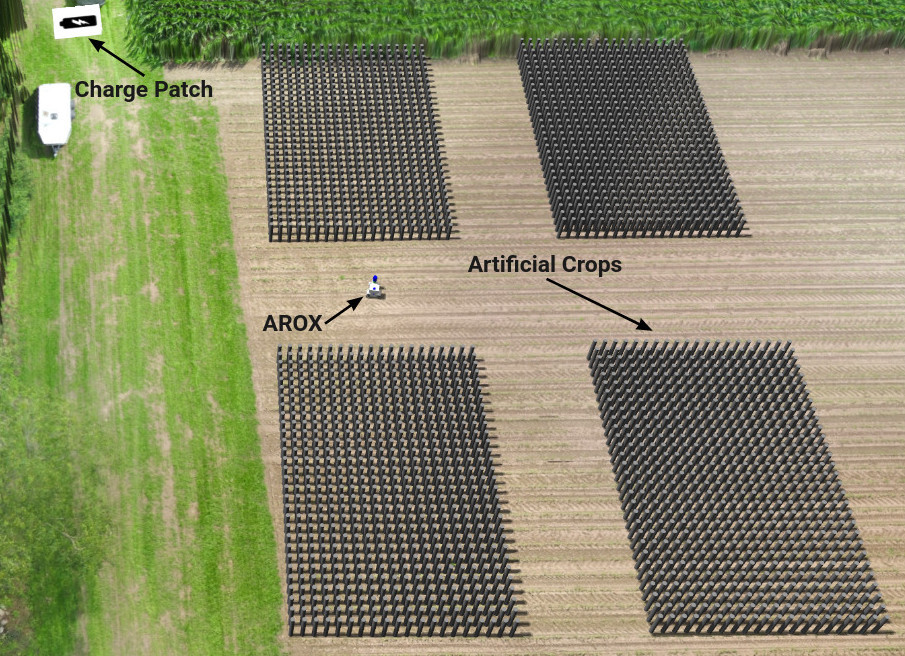
\includegraphics[width=\textwidth]{img/prototype_scenario.jpg}
        \caption{\textsc{Prototypical Layout}}
        \label{fig:prototypical_layout}
    \end{subfigure}
    \hfill
    \begin{subfigure}[b]{0.49\textwidth}
        \centering
        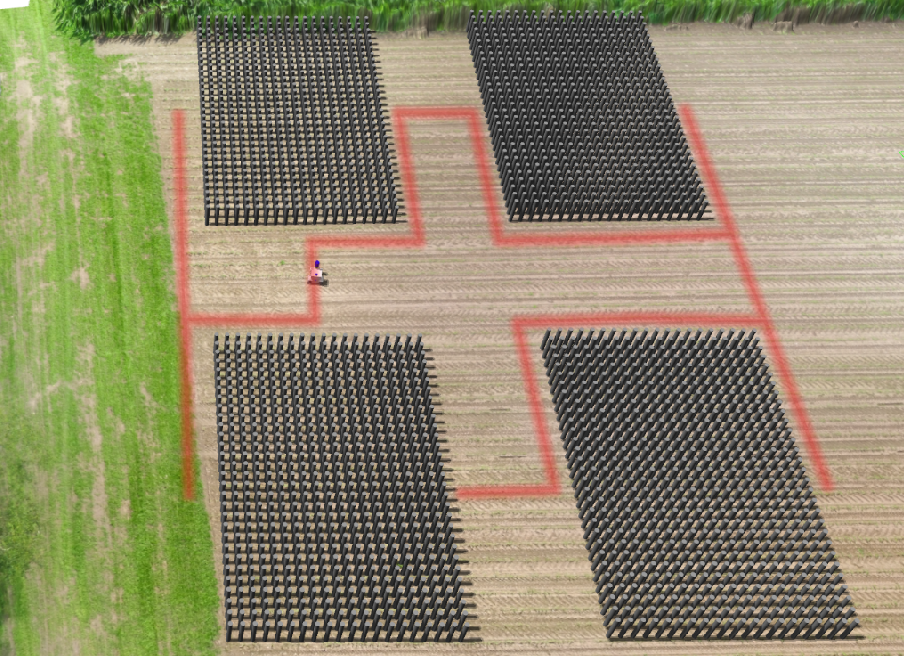
\includegraphics[width=\textwidth]{img/example_path.png}
        \caption{\textsc{Example Scan Route}}
        \label{fig:example_scan_route}
    \end{subfigure}
\caption{\textsc{Prototype Scenario in the Simulation}}
\label{fig:prototype_sim}
\end{figure}

\section{Robotic System and Infrastructure}
\label{sec:robotic_system}

The robotic system under consideration is going to be the \textit{Autonomous Robotic Experimentation Platform} (AROX) \cite{Kisliuk:2021} that is depicted in figure \ref{fig:arox_system}.
It is assumed to integrate all the essential software and hardware required for the task at hand, i.e., processing a given plan (e.g. human provided) that causes the robot
to autonomously drive to specified locations and record scans. As discussed, this should be possible over extended periods of time, i.e., long term, including charge stops, etc.
According to Kunze et al. \cite{Kunze:2018}, different areas of AI must be brought together to enable long-term autonomous robots in practical applications.
As essential building blocks, they identify \textit{navigation \& mapping}, \textit{perception}, \textit{knowledge representation \& reasoning}, \textit{planning},
\textit{interaction}, and \textit{learning}. Correspondingly, all these aspects are in some sense part of the AROX system, some more, some less explicit and sophisticated.
The AROX consists of a two-axle (2WD differential drive) mobile platform based on an \textit{Innok Heros}\footnote{\textcolor{link-color}{\url{https://www.innok-robotics.de/produkte/heros}}}. \cite{Kisliuk:2021}
In addition to the AROX system itself, Kisliuk et al. introduce a supporting infrastructure in the form of a mobile base station (container) at the field site,
which provides an inductive charging station, a mobile internet connection and a WiFi network for local data exchange.
Real-time kinematics (RTK) is used, a differential GNSS\footnote{Global Navigation Satellite System} method that results in high-precision positioning (in centimeter range)
near a base station, such as the mobile container. The errors or inaccuracies of basic GNSS techniques are avoided in RTK solutions by transmitting correction signals based
on carrier measurements of the base station, whose location is precisely known. \cite{RTK_fundamentals} For this purpose, the container also provides an 
NTRIP\footnote{Networked Transport of RTCM (Radio Technical Commission for Maritime Services) via Internet Protocol} server.
Besides these technical features of the container, it also simply serves as a shelter for the robot.
In order to actually use RTK, a real-time communication channel (e.g. WiFi) is needed to connect the RTK base station, i.e., the mobile container, with the RTK rover,
i.e., the AROX, to transmit the aforementioned correction signals. Furthermore, it is crucial that both the robot and the base station receive their own GNSS signals, 
i.e., are connected to the GNSS service. The AROX also maintains WiFi or LTE connections for the purpose of transmitting the recorded scans to external servers or the base station.
The robot's localization is multi-layered and based on sensor fusion of inertial measurement unit (IMU), odometry and RTK-GNSS data using the \code{robot_localization} \cite{Moore:2014} package.
Several laser scanners are attached to its base and used to avoid collisions, e.g., the \textit{SICK TiM} and the \textit{Velodyne Puck} mounted at the optional sensor
slots displayed in fig. \ref{fig:arox_system}. For the actual task of plant monitoring, the high-resolution $3D$ lidar sensor \textit{RIEGL VZ-$400$i} is used,
which can be combined with a calibrated hyperspectral or RGB camera (cf. fig. \ref{fig:arox_system}). \cite{Kisliuk:2021}
For \textit{navigation}, the ROS package \code{move_base_flex} \cite{Puetz:2018} is used, a more flexible extension of the standard ROS navigation framework \code{move_base}\footnote{\textcolor{link-color}{\url{https://wiki.ros.org/move_base}}}.
The primarily used path planning algorithms are provided by the ROS packages \code{eband_local_planner}\footnote{\textcolor{link-color}{\url{https://wiki.ros.org/eband_local_planner}}} and \code{dwa_local_planner}\footnote{\textcolor{link-color}{\url{https://wiki.ros.org/dwa_local_planner}}}.
Effective navigation assumes knowledge of the environment, e.g., a map, so that the robot can estimate its position relative to the navigation target. \cite{Krajnik:2010}
There are numerous approaches to representing knowledge about the environment. The map may be static and such that the robot only needs to be able to locate itself in that
map, or the robot may need to perform simultaneous localization and mapping (SLAM). \cite{Krajnik:2010} Particularly in long-term autonomy scenarios, the robot must be able to cope
with environmental changes over time. Santos et al. propose a way for the robot to update and refine its environment representations during long-term application. \cite{Santos:2016}
They introduce a $4D$ environment representation, i.e., they incorporate the time domain to account for dynamic changes. As introduced in section \ref{sec:prototype_scenario}, the AROX
in the basic configuration assumed in this work does not have an explicit \textit{knowledge representation}, but only a predefined static map of the environment. Moreover, the map
is not updated, i.e., no learning takes place in this sense, and no environmental changes are taken into account. In this simple scenario, \textit{reasoning} is also disregarded.
Another interesting facet is \textit{perception}. There is a kind of perception in the form of obstacle detection based on laser scans, but it is not a particularly elaborate form
of perception. An even less pronounced part of the system is \textit{learning}, technically this aspect also occurs somehow, e.g., in the sense that obstacles are detected and entered
into the local costmap. Of course,
sensor information is transferred into a kind of knowledge representation, so in a way obstacles in the environment are learned. Nevertheless, this is not what is typically
understood by machine learning. A counterexample is \textit{interaction}, which is again very explicitly part of the scenario under consideration, namely in the form of communication and
cooperation with the human operator (cf. section \ref{sec:fallback_solution}). The \textit{planning} process itself is not part of the scenario, but it is assumed that plans are available and usable,
e.g., handcrafted by a human operator or generated by a planner from the literature. In further extensions, all these aspects will play a more important role, as useful applications
have already been identified that could improve the long-term autonomy performance of the system in the future, but not in the minimum long-term autonomy scenario considered in this
thesis. To sum up: Technically, all of the aspects proposed by Kunze et al. are somewhat necessary and part of the system, but in part only in a very basal fashion. Certain aspects
are simply not explicitly part of the application. In addition to the actual physically available AROX, the system has been modeled in the unified robot description format (URDF) and
can be used in a simulation (cf. fig. \ref{fig:prototypical_layout}).
\begin{figure}[H]
    \centering
    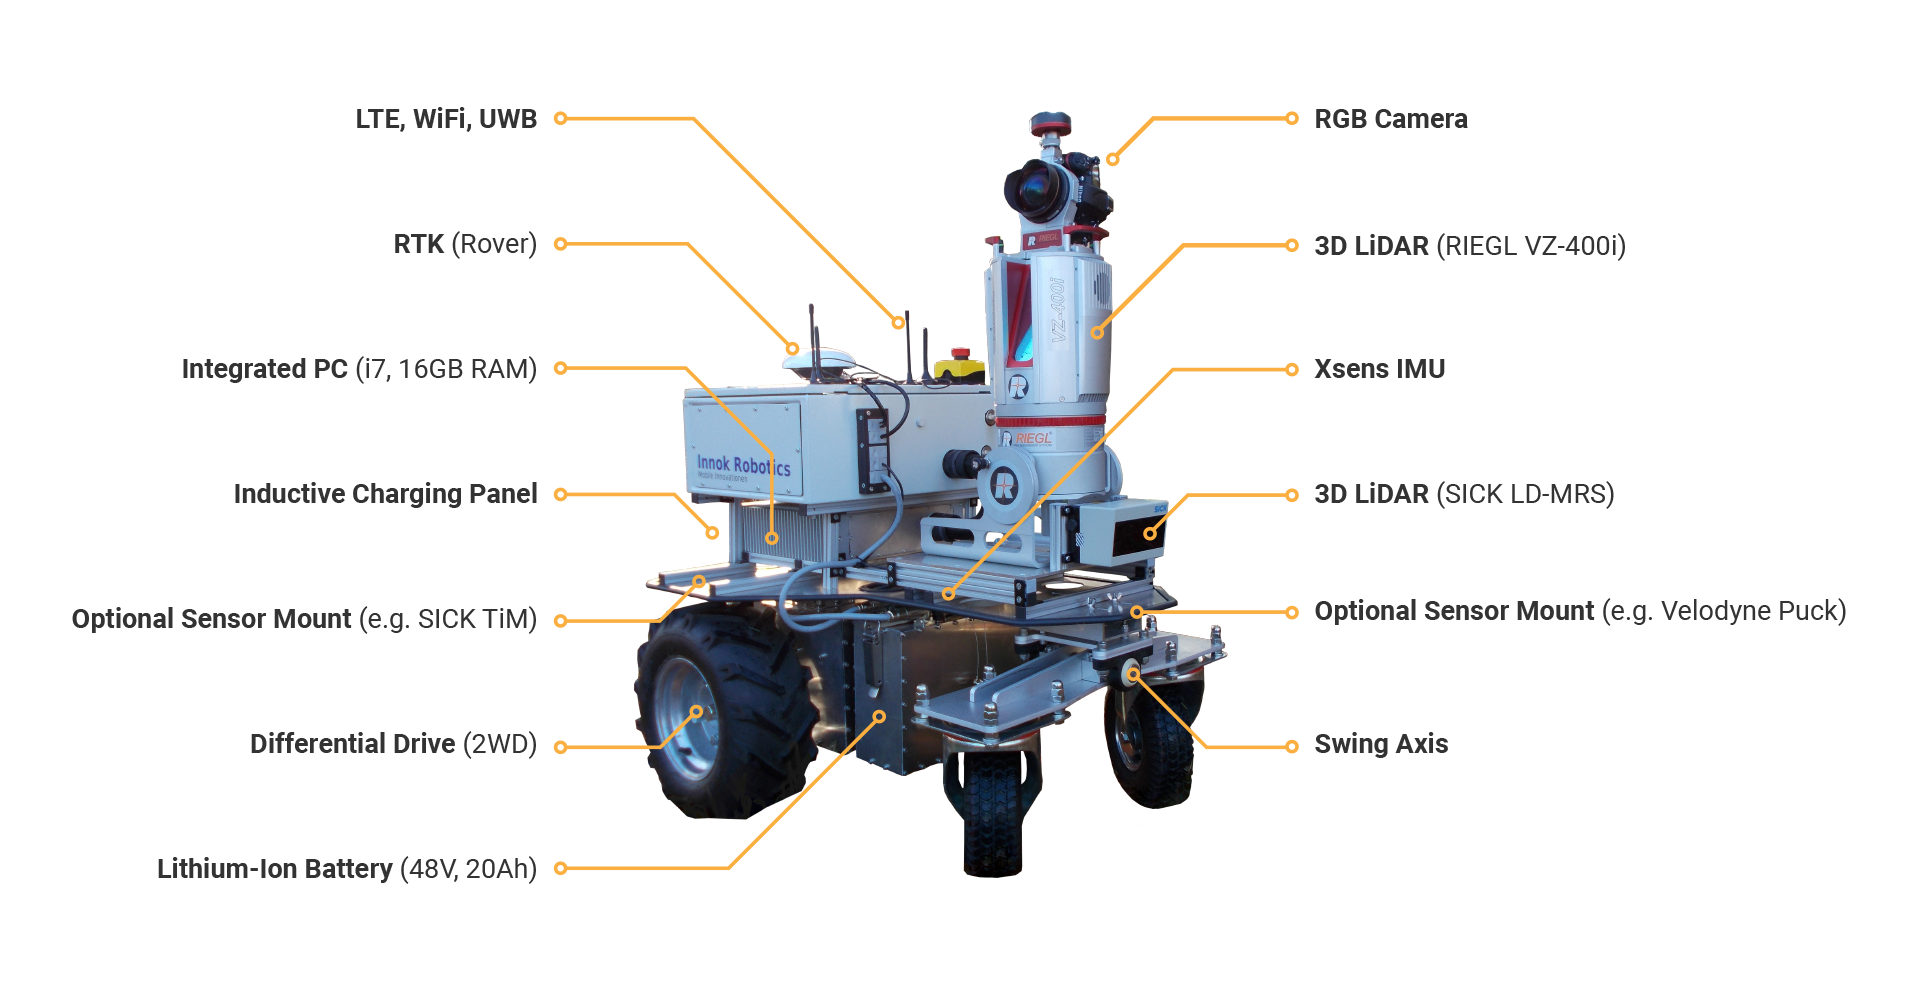
\includegraphics[width=\textwidth]{img/robot_description_smaller.png}
    \caption{\textsc{Autonomous Robotic Experimentation Platform (AROX)}}
    \label{fig:arox_system}
\end{figure}

\section{Challenges for Long-Term Autonomy}
\label{sec:challenges_for_lta}

Having clarified what long-term autonomy (LTA) means for this work, we now turn to potential problems that stand in its way.
There are numerous potential hinderances for long-term autonomous systems that can cause failure and prevent the system from continuing its task.
The following three constraints precisely define the LTA problems considered in this work.
\begin{enumerate}
    \item It can practically occur in the concrete scenario described in sections \ref{sec:lta_plant_observation} and \ref{sec:prototype_scenario}.
    \item It can prevent the smooth functioning of an LTA system or affect the quality of its results.
    \item It can be detected by monitoring methods and subsequently solved or communicated.
\end{enumerate}
This definition contains certain implicit assumptions. The first constraint, for example, implies that these problems should have some probability of occurring,
i.e., they should be relatively likely to occur. Accordingly, potential problems such as lightning strikes or wild boar attacks are ignored because they are highly 
unlikely and also difficult, if not impossible, to solve. Moreover, many of the issues of this rather unconventional type, if solvable, could in principle be covered
by more general classes of issues from the following list. Furthermore, the third constraint, i.e., that the considered problems can be detected and subsequently solved 
or communicated, assumes that the system is still fundamentally functioning and has not completely collapsed; a counterexample would again be a lightning strike.
Without claiming to be exhaustive, the following is a list of potential challenges in an agricultural field monitoring context that, 
from a practical perspective, fulfill the above restrictions and are thus worthy of investigation:
\begin{itemize}
    \item \textbf{power management} - battery failure, unexpected low battery
    \item \textbf{charging failure} - unsuccessful docking, no charging
    \item \textbf{drastic weather change} - storm, fog, heavy rain, extreme cold
    \item \textbf{certain dynamics} - day, night
    \item \textbf{sensor (perception) failure}
    \item \textbf{perceptual aliasing issue}
    \item \textbf{data management} - full memory, sensor data processing failure
    \item \textbf{lost connection} - WiFi, RTK-GNSS, internet
    \item \textbf{obstacles blocking planned path} - static, dynamic
    \item \textbf{robot gets stuck} - spinning wheels
    \item \textbf{robot falls over}
    \item \textbf{navigation failure} - \code{move_base_flex}
    \item \textbf{sustained recovery} - no return to normal operation
    \item \textbf{incorrect / inaccurate localization} - IMU, odometry, GNSS
    \item \textbf{mapping error} - incorrect costmap entries
    \item \textbf{plan deployment failure} - robot remains in idle state
\end{itemize}
When trying to envision challenges for long-term autonomous application of mobile robots, a common approach is to simply run a robot in such an environment for extended periods
of time and log any information that might somehow be relevant and indicative of problems, e.g., sensor data, internal diagnostics, etc. \cite{Biswas:2016}
Some of the challenges from the above list result from attempts of this type or the coincidental occurrence in other experiments. Others are obviously potential problems that may occur
and do not require further evidence or justification. The last group is the result of extensive literature research, i.e., challenges encountered in long-term autonomous experiments
presented in the literature. For each potential issue identified, its relevance and consequences, i.e., a brief description of why it might be problematic, is provided in section \ref{sec:brief_overview_challenges}.
A more detailed consideration as well as monitoring and simulation approaches are presented in section \ref{sec:sim_and_mon_of_lta_challenges}.

\subsection{Brief Overview of the Identified Problem Categories}
\label{sec:brief_overview_challenges}

For each potential problem identified in the last section, its relevance and implications, i.e., a brief description of why it might be problematic, is provided below.\newline

\noindent
\textbf{Power Management}\newline

\noindent
A natural requirement for LTA systems as defined in section \ref{sec:lta_plant_observation} is some form of energy management.
The system is expected to operate autonomously for extended periods of time, which of course assumes a power supply. 
As Hawes et al. \cite{Hawes:2017} point out, managing consumable resources such as battery charge is critical to long-term autonomous systems.
However, the energy management estimated at planning time may not work correctly or as expected at execution time, e.g., the battery could be 
depleted before the planned time. Or worse, there could be a complete battery failure. It would certainly be useful to enable the system to handle such issues, at least to 
some degree. Arvin et al. point out that long-term autonomy experiments are still rare due to the limited battery capacity of robots. \cite{Arvin:2018}
Therefore, they believe that solving power management issues is of great importance.\newline

\noindent
\textbf{Charging Failure}\newline

\noindent
Another category of potential LTA problems related to the system's power supply is charging failures. Several things can go wrong during a charging process. 
Leaving aside the simplistic assumption of charging upon arrival at specific coordinates and considering the actual charging process 
in practice with the AROX system, it must dock with an inductive charging station in a mobile container at the field site.
Accordingly, docking to the charging station may fail or the charging process itself may not start after docking.
Both cases lead to a failed charging process and thus to an abortion of the robot's LTA mission.
There is evidence in the literature that this is a common problem in long-term autonomous operation of mobile robots. Wang et al. \cite{Wang:2018}, for instance, encountered
this problem during the deployment of their long-term autonomous service robots when the charging port failed and the robot could not recharge and thus continue its mission.
An evaluation of potential docking failures requires the integration of the autonomous docking / undocking solution described in section \ref{sec:docking_solution}.\newline

\noindent
\textbf{Drastic Weather Change}\newline

\noindent
Since the AROX system is designed for moderate weather conditions, drastic weather changes can also play a role.
If the weather changes too drastically, it can be problematic for various aspects of the system.
If it is stormy, for example, this can be delicate for the sensor recordings, but also for the robot platform itself, as it could fall over or otherwise be damaged.
The quality of the sensor images can also be affected by fog or extreme sunlight (illumination).
In addition, heavy rain should also be avoided. Finally, extreme cold could be a major problem for the system's battery.\newline

\noindent
\textbf{Certain Dynamics}\newline

\noindent
Similar to weather changes, there are other dynamics such as the natural transition from day to night. For sunlight-dependent sensors such as cameras, 
the robot should take twilight into account and plan its operations accordingly to be back in the shelter, i.e., the mobile container, by dark.\newline

\noindent
\textbf{Sensor (Perception) Failure}\newline

\noindent
Hardware issues are a very general problem class and could relate to almost arbitrary many kinds of problems. Since the correct functioning of the $3D$ lidar sensor is
crucial for the long-term monitoring scenario described in section \ref{sec:lta_plant_observation}, the main focus will be on detecting hardware faults of this type. 
Sensor failures are, of course, a failure class in which the robot can do little except attempt to restart the corresponding sensor, and therefore rarely has any choice but to 
call the human operator for assistance. Nevertheless, it is important to identify such a malfunction as soon as possible, communicate the problem and avoid a lot of useless work 
and wasted operating time.\newline

\noindent
\textbf{Perceptual Aliasing Issue}\newline

\noindent
Place recognition can certainly be useful for LTA operation of a mobile robot. However, long-term place recognition is not trivial because 
the appearance of places in the environment changes quite drastically over time, e.g., due to illumination, vegetation periods, or weather. \cite{Han:2018}
A useful approach to compare two images (places) is local feature matching, e.g., based on the \textit{Scale-Invariant Feature Transform (SIFT)} and
\textit{Speeded Up Robust Features (SURF)} algorithms. \cite{Valgren:2007} The authors discuss how such approaches can be facilitated to address the problems related to drastic
environment changes. Another method, proposed by Neubert et al. \cite{Neubert:2013} attempts to predict environmental appearance changes based on the assumption that they are
often systematic and repeatable. Moreover, Latif et al. tackle the task of place recognition using \textit{Generative Adversarial Networks (GANs)}, which enable them to transform the appearance, e.g., from summer
to winter, without requiring knowledge of the image correspondence beforehand, ending up with different versions of an environment snapshot in which the structure remains the same.
\cite{Latif:2018} These versions can then be used to learn how to distinguish locations. A further approach to recognizing changes between observations is based on the idea of
learning to separate the static and dynamic structures of an environment during long-term deployments. \cite{Ambrus:2014}
Visual place recognition in changing environments is a very active area of research, where it is far beyond the scope of this thesis to cover all recent advances (cf. \cite{Porav:2018},
\cite{LowrySur:2016}, \cite{Suenderhauf:2013}, \cite{Lowry:2016}, \cite{Milford:2012}, \cite{Churchill:2013}). In the scenario considered in this work, it is particularly relevant that the robot is able to recognize the place of the mobile container
that serves as shelter and provides the charging station. In addition to the natural changes in the environment over time, there is another important aspect
that makes long-term place recognition particularly challenging - the perceptual aliasing issue. This problem refers to the fact that certain places and objects are very 
similar to each other, that is, they have many common characteristics, which makes them hard to distinguish. \cite{Han:2018}
If, for example, a mobile office container is placed right next to the robot's base station, it might be difficult for the robot to distinguish the objects.
Hence, there could be a need for monitoring methods that are capable of recognizing such situations and providing some strategies to resolve the perceptual aliasing issue.\newline

\noindent
\textbf{Data Management}\newline

\noindent
As robots are deployed for increasingly long periods of time (LTA), it becomes ever more essential to address the challenge of managing the vast amounts of data that are generated
during such deployments. \cite{Ambrus:2014} Since the overall objective of the robot's missions is to acquire data, the appropriate management of this data is of relevance.
If, for example, the robot is no longer able to save further scans due to a full memory, it should recognize and communicate this.
In addition, there may be disturbances in the processing of the sensor data, so that the robot is no longer able to process and save the recordings correctly.
Successful scanning is worthless if the resulting data is not saved properly, so it is important to monitor whether the scans are being written to a file correctly.
Therefore, it would be valuable to identify such problems as soon as possible to avoid redundant missions.\newline

\noindent
\textbf{Lost Connection}\newline

\noindent
For the robot to work as expected, it must maintain connections to various services. Accordingly, an interruption of one of these connections should be detected immediately.
A real time communication channel (e.g. WiFi) is required to connect the RTK base station, i.e., the mobile container, and the RTK rover, i.e., the robot, in order to
transmit the correction signals for high-precision positioning. In the literature, there are several examples of (semi-)autonomous mobile robots that cannot continue their
mission as expected when they lose WiFi connectivity, such as the service robots considered by Wang et al. \cite{Wang:2018}. The authors also establish a form of network monitoring
to deal with disconnects.
Furthermore, it is crucial that both the robot and the base station receive their own GNSS signals,
i.e., are connected to the GNSS service. Bargoti et al. \cite{Bargoti:2015} and Bechar et al. \cite{Bechar:2016} identify occlusion of GPS satellites leading to jumps in estimated position as one of the main reasons
for detection failures in their tree monitoring scenario, which highlights the value of being able to detect poor GNSS links.
In addition, the RTK-GNSS data is used for scan registration. Finally, the recorded scans are transmitted via WiFi or LTE 
to the base station or external servers for further processing. Whether LTE is behind it or the internet connection is provided via WiFi, it would make sense
to monitor the robot's internet connection in any case. For all connections, it is not only about complete disconnects, but also about qualitative estimations.\newline

\noindent
\textbf{Obstacles Blocking the Planned Path}\newline

\noindent
A relatively common problem for the long-term autonomy of a mobile robot is obstacles blocking the planned path.
A rough distinction can be made between static obstacles such as a trailer and dynamic obstacles such as animals or people.
Wang et al. \cite{Wang:2018} even claim that the greatest challenge for the navigation of autonomous robots are dynamic obstacles.
The used navigation framework \code{move_base_flex} can already detect obstacles and initiate a recovery behavior if the planned path is not traversable.
However, it would be good to refine the default recovery behaviors and adapt them to the scenario at hand. In addition, the robot should be able to deal with
recovery failures.\newline

\noindent
\textbf{Robot Gets Stuck}\newline

\noindent
A problem not unlike the obstacles, but slightly different, is that the robot gets stuck and cannot move on. This can happen, for example, when the wheels spin due 
to a muddy path. Such situations where the robot cannot move even though the plan calls for it should be identified and addressed.\newline

\noindent
\textbf{Robot Falls Over}\newline

\noindent
A special case of getting stuck, which should nevertheless be considered separately, is the robot falling over.
This issue should be considered separately, since in such a case the robot will not be able to recover and continue its mission without human assistance in any case.\newline

\noindent
\textbf{Navigation Failure}\newline

\noindent
Another potential LTA problem category, under which a whole range of concrete problems are subsumed, and which have already been encountered in experiments conducted as part of
this work, are navigation errors, which pose a particular challenge in highly dynamic real-world environments. \cite{DelDuchetto:2018}
For example, the local planner configured in \code{move_base_flex} (e.g. DWA, EBand) provides a path that
is infeasible, e.g., tries to drive around a field,  although there is no way. Del Duchetto et al. encounter similar issues in an indoor LTA scenario where valid navigation
trajectories cannot be generated from time to time.
They establish specific, hard-coded ad-hoc recovery behaviors for such cases, ranging from simple wait-and-repeat to interactive human assistance. \cite{DelDuchetto:2018} As Hawes
et al. \cite{Hawes:2017} point out, navigation errors are a critical factor for the long-term autonomy of a mobile robot, as they can render the robot incapable of driving back
to the charging station (mobile container). Hence, it is imperative to guarantee a certain level of robustness against navigational flaws, i.e., to provide the robot with the
ability to detect and recover from such errors. \cite{DelDuchetto:2018}
The authors define the errors as follows: \textquote{\textit{[...] situation in which the robot is not able to progress toward the goal, because it is not
moving or it is performing some counterproductive behavior}}. \cite{DelDuchetto:2018}
As introduced in section \ref{sec:robotic_system}, the navigation system used is \code{move_base_flex}, an extension of the common ROS navigation framework \code{move_base}.
Navigation issues in practice can be due to a variety of reasons, such as sensor noise, dynamic obstacles, or inaccurate controls \cite{DelDuchetto:2018} and some of them are already
detected by \code{move_base_flex}. Nevertheless, even if this is the case, this information must still be used and processed appropriately by the system in order to be dealt with.\newline

\noindent
\textbf{Sustained Recovery}\newline

\noindent
If the robot tries to recover from a problematic situation, e.g., obstacles on the planned path, such a recovery may not be successful, i.e., the robot may not be able
to return to the normal operation state. In case of an unsuccessful recovery attempt, the robot could either give up and abort its mission or perform another recovery.
Of course, the robot should not end up in an infinite loop of repeating the same failing recovery, but instead it should try a few different recovery attempts,
and if none of them work, it should shut down and call the operator. Therefore, it is important to introduce monitoring solutions for recovery behaviors as well.\newline

\noindent
\textbf{Incorrect or Inaccurate Localization}\newline

\noindent
It is obvious that it is a problem when the robot is not able to localize itself correctly in its environment.
Localization is a critical factor for a robot's long-term autonomy, which should therefore not deteriorate during long-term deployments. \cite{Hawes:2017}
In this case, it is a matter of localization within a global reference system, i.e., determining the pose (position and orientation) within a given map of the environment.
If the localization is no longer accurate, e.g., because the robot has been moved to a different position in the map, it must detect this in order to
trigger relocalization. In the case of such a localization error, the \textit{kidnapped robot problem} arises, because although no one has 
physically removed the robot from its position, it appears that way from the robot's perspective. \cite{Hertzberg:2012}
The relevance here can easily be argued based on practical experience, as this issue has already caused a lot of trouble in practice with the AROX system during 
the work for the \textit{PORTAL} project. In these situations, a major challenge for localization was rotating the robot on the spot.
The problems encountered consisted mostly of an incorrect orientation of the robot and rather rarely of an actual incorrect position.
If the orientation is incorrect, the sensor records will also be incorrectly aligned, which is a major issue for the scenario under consideration.
In addition to this practical experience, there are also numerous references in the literature to localization problems in long-term autonomous robot operations. For instance,
Wang et al. \cite{Wang:2018}, who identified localization and execution errors as the two core challenges in their long-term application of indoor service robots.
They identify unexpected changes in the robot's position estimates as a useful method for predicting / detecting localization problems.
Of course, it can also be a problem for localization if the GNSS signal itself is inaccurate or non-existent \cite{Churchill:2013}, but that is another topic (cf. \textit{Lost Connection} section).
There are arbitrary many potential localization issues (e.g. slipping in sand, getting stuck, jammed wheels) and the correct functioning of the system always assumes an accurate
position estimate. \cite{Goldberg:2002}\newline

\noindent
\textbf{Mapping Issues}\newline

\noindent
Mapping issues can generally refer to a variety of problems. In this case, a particular issue regarding the local \textit{costmap} observed during experiments for this work is meant.
The \textit{costmap} is a $2D$ occupancy grid based on sensor data of the world. It generates costs based on a user defined inflation radius.
If the robot drives over a hill and the sensors are configured in a certain way, parts of the ground may be incorrectly perceived as an obstacle and entered into the \textit{costmap}.
The challenge then is that the robot is unable to drive through these ``virtual'' obstacles.\newline

\noindent
\textbf{Plan Deployment Failure}\newline

\noindent
The last type of problem is rather trivial again. If the plan distribution node does not provide a plan for the robot to execute, it remains idle until a human operator 
notices and takes care of it. It might therefore be useful to let the operator know if a plan has still not arrived after a certain time.
In addition, faulty plans that are not executable should also be reported, which requires some kind of content plausibility check.\newline

\noindent
\textit{Concluding Remarks}\newline

\noindent
The idea is to tackle a subset of this list of issues that is realistically solvable in the scope of the work.
Generally, the potential barriers for long-term autonomy can be classified into three categories of increasing negative impact on the system:
\begin{figure}[H]
\centering
\begin{enumerate}
    \item The robot recognizes a problem and is able to solve it by itself.
    \item The robot recognizes a problem, is unable to solve it, and calls an operator for help.
    \item The robot has a malfunction / problem, does not recognize it and therefore cannot solve or communicate it.
\end{enumerate}
\caption{\textsc{Classification of Problems in Terms of Impact}}
\label{fig:problem_types}
\end{figure}
\noindent
Type $(1)$ is the ideal case and accordingly the ultimate goal of all efforts to implement long-term autonomy in practice. Type $(2)$ is already a step forward, because problems
are at least recognized and can be communicated, which is the minimum requirement to guarantee a certain robustness with respect to the problems.
In the baseline scenario, i.e., the running prototype of an integrated solution, each potential issue in the above list is classified as type $(3)$.
Part of the goal of this work is to shift the challenges of the selected subset to another category and thereby improve the utility of the system, 
i.e., to solve them completely $(1)$, or at least to enable the robot to recognize them with execution monitoring approaches and request help $(2)$.
However, it is also part of the truth that not all possible external influences are solvable, i.e., a robot will not be able to solve all
conceivable problems itself. Long-term autonomy has its limits, and there are simply unpredictable situations that a mobile robot cannot be expected to handle,
e.g., if its battery bursts into flames, or it is knocked over by something. In such a case, the only way to do damage control is to try to shut down the 
robot in a controlled manner (e.g. with data backup) and, if possible, communicate the problem.
Of course, one could assign probabilities to specific incidents, which vary depending on the information available. 
For example, if the robot detects that the battery is showing unusual discharge behavior, such information could be taken into account and 
reported to the operator. Nevertheless, it is not feasible to cover everything that can happen, and long-term autonomy is subject to certain limits.

\subsection{Relevance Assessment}
\label{sec:relevance_assessment}

To assess the relevance of the potential challenges to long-term autonomy introduced in the last section, a kind of informal analysis of the impact,
difficulty, and likelihood of each problem was conducted. The idea is not to arbitrarily select the challenges that will be studied in more detail as part
of this work, but to rely on the judgment of the more experienced roboticists in the working group, especially those who have hands-on experience with the
AROX or similar systems, to set priorities. For this purpose, a simple questionnaire was designed in the form of a spreadsheet. The first aspect by which participants
were asked to rank each problem was its respective impact from \textit{high} ($1$), i.e., prevents a successful mission, to \textit{medium} ($2$) impact, e.g., delays missions
or reduces the quality of results, to \textit{low} ($3$), where it has at most a minor impact on the robot's mission. The next aspect was about evaluating each issue in
terms of its individual difficulty of solution and recognition. The options were \textit{easy} ($1$), meaning that simple solutions exist, \textit{medium} ($2$), which
requires some effort but should be feasible within the scope of the work, to \textit{hard} ($3$), i.e., that it is a rather general issue that can only be tackled in first
approximation. Finally, the likelihood of each problem occurring should be evaluated using the following three options. \textit{Very likely} ($1$), which roughly means it has been
experienced in practice several times, \textit{occurs} ($2$), which means it has been experienced or heard of once, and \textit{highly unlikely} ($3$), which means it has never been
heard of. The questionnaire was completed by a total of $7$ people. Obviously, this can by no means be considered representative or significant, but it
nevertheless does give an indication of which challenges should be considered with higher priority and contributes to systematization. The accumulated results are visualized in the
$3D$ scatter plot depicted in figure \ref{fig:questionnaire_results}. For each issue, the average vote among all three dimensions (impact, difficulty, likelihood) is displayed.
The most relevant problem to consider under the introduced scoring system would be a problem at coordinates $(1, 1, 1)$, i.e., a high-impact problem 
that is easy to solve / discover and has a high probability of occurring. This optimal combination is shown as a golden cross in figure \ref{fig:questionnaire_results}.
The challenges closest to this point in $3D$ space are the ones that are most important to consider based on the questionnaire and therefore should be 
investigated with higher priority in this work. For a more detailed overview, the average results and each problem's distance to the optimum can be taken from the table 
in figure \ref{fig:average_results}.

\vfill
\pagebreak

\begin{figure}[H]
    \centering
    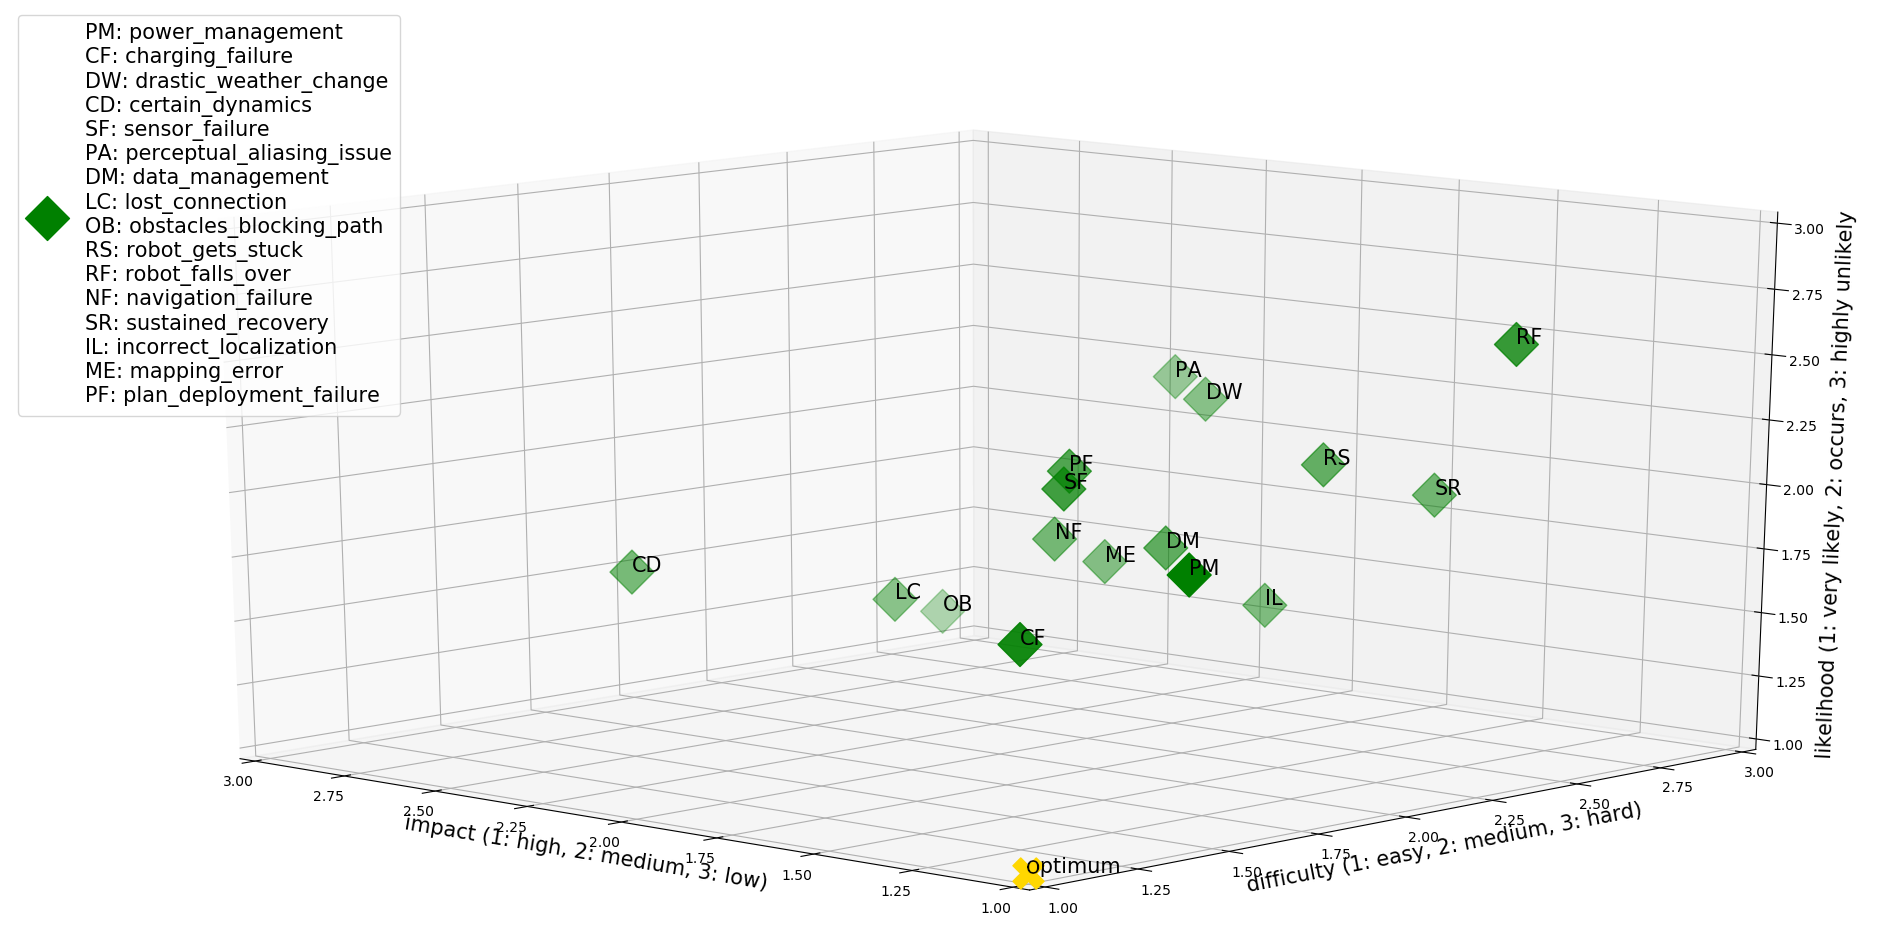
\includegraphics[width=0.9\textwidth]{img/questionnaire.png}
    \caption{\textsc{Accumulated Results of Questionnaire}}
    \label{fig:questionnaire_results}
\end{figure}
\noindent
The results shown in the table in fig. \ref{fig:average_results} are ordered by their relevance according to the questionnaire results, i.e.,
by their distance from the optimal combination of impact, difficulty, and likelihood. It is worth mentioning, however, that the resulting order is based on the assumption
that the three criteria of impact, difficulty, and likelihood are equally important in the consideration. One could argue that the difficulty criterion was introduced 
primarily because of the tight time frame of this work and may be less important when it comes to the question of which problem is really crucial to solve in practice.
Thus, it is worth considering the two-dimensional results only in terms of the expected impact and likelihood of each problem displayed in fig. \ref{fig:questionnaire_results_2d}.
\begin{figure}[H]
    \centering
    \resizebox{0.7\textwidth}{!}{
    \begin{tabular}{| c | c | c | c | c |}
        \hline
        \textbf{problem} & \textbf{\o \thinspace impact} & \textbf{\o \thinspace difficulty} & \textbf{\o \thinspace likelihood} & \textbf{dist. to optimum} \\ \hline
        charging\_failure & $1.29$ & $1.29$ & $1.71$ & $0.82$ \\ \hline
        power\_management & $1.0$ & $1.43$ & $2.0$ & $1.09$ \\ \hline
        data\_management & $1.57$ & $2.0$ & $1.86$ & $1.44$ \\ \hline
        sensor\_failure & $1.57$ & $1.71$ & $2.14$ & $1.46$ \\ \hline
        incorrect\_localization & $1.57$ & $2.29$ & $1.57$ & $1.52$ \\ \hline
        lost\_connection & $2.14$ & $1.86$ & $1.57$ & $1.54$ \\ \hline
        navigation\_failure & $1.86$ & $2.0$ & $1.83$ & $1.56$ \\ \hline
        plan\_deployment\_failure & $1.67$ & $1.83$ & $2.17$ & $1.58$ \\ \hline
        mapping\_error & $1.86$ & $2.14$ & $1.71$ & $1.6$ \\ \hline
        certain\_dynamics & $2.43$ & $1.43$ & $1.71$ & $1.65$ \\ \hline
        obstacles\_blocking\_path & $2.29$ & $2.14$ & $1.43$ & $1.77$ \\ \hline
        robot\_gets\_stuck & $1.43$ & $2.29$ & $2.14$ & $1.77$ \\ \hline
        sustained\_recovery & $1.33$ & $2.5$ & $2.0$ & $1.83$ \\ \hline
        drastic\_weather\_change & $1.86$ & $2.43$ & $2.29$ & $2.11$ \\ \hline
        robot\_falls\_over & $1.0$ & $2.33$ & $2.67$ & $2.13$ \\ \hline
        perceptual\_aliasing\_issue & $2.0$ & $2.5$ & $2.33$ & $2.24$ \\ \hline
    \end{tabular}}
\caption{\textsc{Results of the Evaluation - Problems Ordered by Relevance}}
\label{fig:average_results}
\end{figure}
\begin{figure}[H]
    \centering
    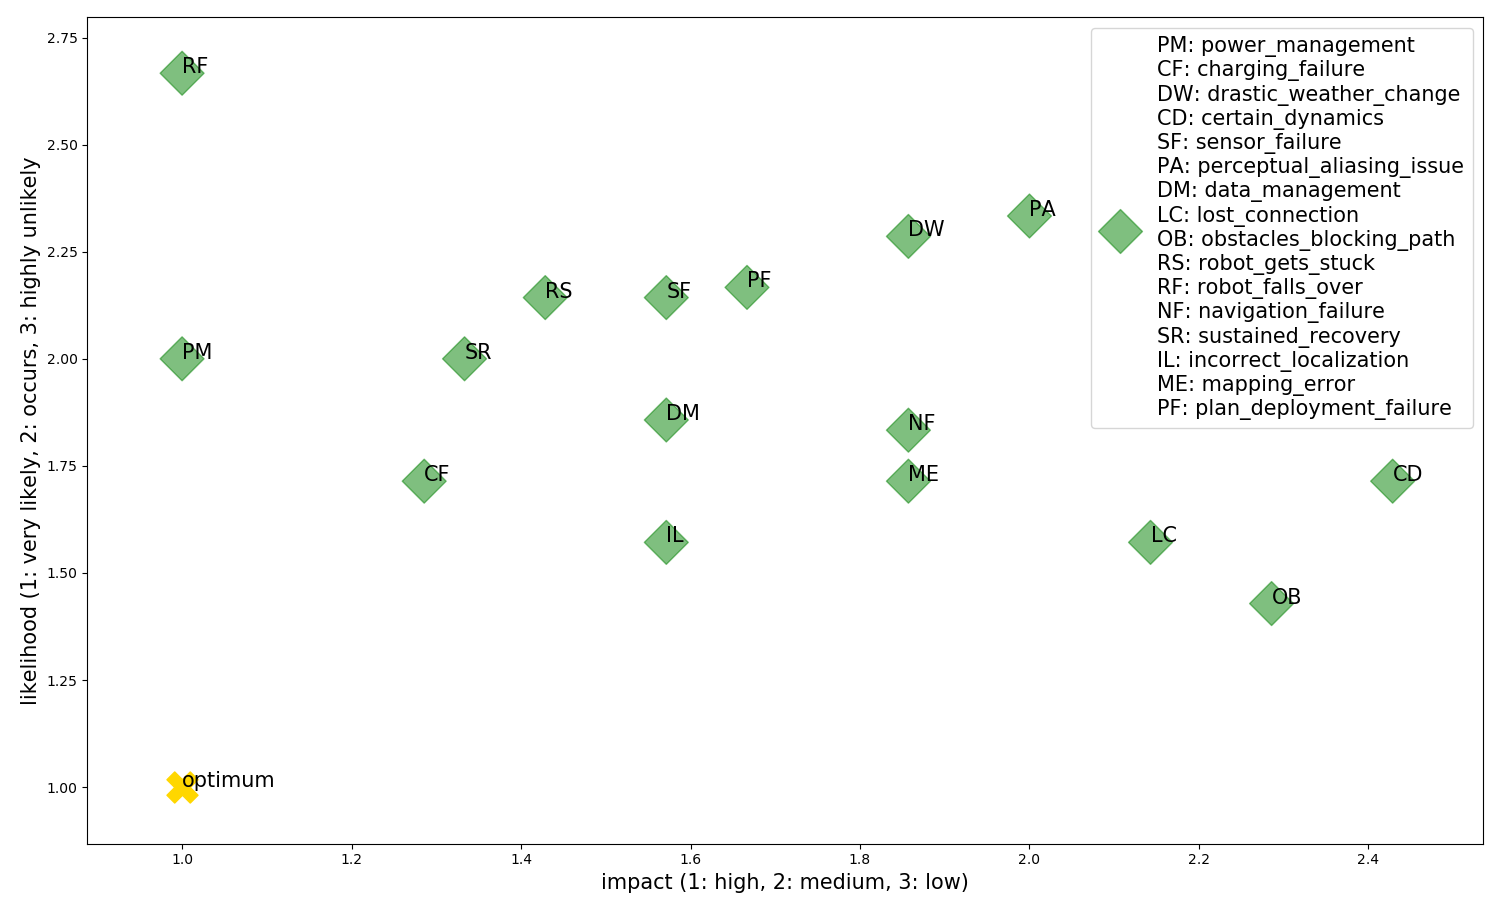
\includegraphics[width=0.8\textwidth]{img/questionnaire_2d.png}
    \caption{\textsc{$2D$ Results of Questionnaire}}
    \label{fig:questionnaire_results_2d}
\end{figure}
\noindent
Another interesting aspect to analyze is the range in given answers in the questionnaire, i.e., the agreement among the participants. Most of the judgments roughly coincide with
only few outliers. However, there are some controversial cases that are worth mentioning. First, the \textit{impact} category seems to be the easiest to assess, as it is the only
one where all participants agreed on two problem types (power management, robot falls over). In addition, the other problem types in the \textit{impact} category are rated fairly
consistently, most of them have only one outlier vote, and it is very rare that the votes are completely mixed. The most contested problem types in this category are perceptual
aliasing, connection losses, situations where the robot gets stuck, and navigation failures. It is also interesting to examine the reason for the mixed results. This could be
because most participants rated the problem as average on the scale, but it could also arise from extreme answers canceling each other out. There is a big difference - one means
participants agree, the other means they do not. For the \textit{impact} category, participants seem to agree overall, with only a few outliers and even some cases of perfect
agreement with unanimous votes. The next category, \textit{difficulty}, is already not so clear-cut, which may be explained by the fact that participants could imagine different
depths of problem-solving based on their particular experience, while \textit{impact} is quite easy to think about. There is no unanimous vote, and there are even some cases where
the answers are very mixed, such as in the case of lost connections, where the answers are almost evenly distributed among the possible options. However, this is still rare, in most
cases the overall trend is clear. Finally, the voting in the third category \textit{likelihood} is similar to the \textit{difficulty} votes. Once again, there is no unanimous vote, but there
are cases where participants are pretty much in agreement, such as in data management failures, where all but one voted for $2$ (\textit{occurs}). There is no extreme example of
evenly distributed responses, most have some tendency and a few outliers. In summary, an average score almost never results from an even distribution of responses across the options,
but almost always results from the actual rating of the problem as average based on the criteria. The exact results can be taken from the appendix 
(cf. section \ref{sec:detailed_questionnaire_results}). As shown in fig. \ref{fig:average_results_2d}, the $2D$ evaluation purely based on impact and likelihood results in a different ordering based on their distances 
to the $2D$ optimum $(1, 1)$.
\begin{figure}[H]
    \centering
    \resizebox{0.6\textwidth}{!}{
    \begin{tabular}{| c | c | c | c | c |}
        \hline
        \textbf{problem} & \textbf{\o \thinspace impact} & \textbf{\o \thinspace likelihood} & \textbf{dist. to optimum} \\ \hline
        charging\_failure & $1.29$ & $1.71$ & $0.77$ \\ \hline
        incorrect\_localization & $1.57$ & $1.57$ & $0.81$ \\ \hline
        power\_management & $1.0$ & $2.0$ & $1.0$ \\ \hline
        data\_management & $1.57$ & $1.86$ & $1.03$ \\ \hline
        sustained\_recovery & $1.33$ & $2.0$ & $1.05$ \\ \hline
        mapping\_error & $1.86$ & $1.71$ & $1.12$ \\ \hline
        navigation\_failure & $1.86$ & $1.83$ & $1.2$ \\ \hline
        robot\_gets\_stuck & $1.43$ & $2.14$ & $1.22$ \\ \hline
        sensor\_failure & $1.57$ & $2.14$ & $1.28$ \\ \hline
        lost\_connection & $2.14$ & $1.57$ & $1.28$ \\ \hline
        plan\_deployment\_failure & $1.67$ & $2.17$ & $1.34$ \\ \hline
        obstacles\_blocking\_path & $2.29$ & $1.43$ & $1.36$ \\ \hline
        drastic\_weather\_change & $1.86$ & $2.29$ & $1.55$ \\ \hline
        certain\_dynamics & $2.43$ & $1.71$ & $1.6$ \\ \hline        
        robot\_falls\_over & $1.0$ & $2.67$ & $1.67$ \\ \hline
        perceptual\_aliasing\_issue & $2.0$ & $2.33$ & $1.67$ \\ \hline
    \end{tabular}}
\caption{\textsc{Results of the $2D$ Evaluation - Problems Ordered by Relevance}}
\label{fig:average_results_2d}
\end{figure}
\noindent
First, it is interesting to note that the charging failure is undisputedly in first place in both the two-dimensional and three-dimensional evaluations.
The challenge of incorrect localization climbs to second place if the difficulty criterion is disregarded. This is followed, as before, by power and data management.
Subsequently, sustained recovery makes a huge jump of eight places when leaving aside its assumed difficulty to detect and solve.
Mapping errors are also on the rise, overtaking sensor failures, lost connections, navigation failures, and plan deployment errors.
Another interesting aspect is that sensor failures are far less relevant when disregarding their surprisingly low rated difficulty.
The remaining challenges remain broadly similar in their assessment, with some changing places in the middle of the list, but this is not so relevant.
The problems rated as least relevant in the questionnaire remain the same as in the $3D$ case, mainly because they are considered relatively unlikely.
In conclusion, both lists are used to prioritize the issues to be studied in this work, as it is of course useful to also consider the difficulty of 
solving these problems, but the $2D$ view can be helpful in case of doubt.\newline

\noindent
Of course, in principle it would be of interest to experimentally evaluate how often these problems occur in reality, but that actually requires elaborate long-term autonomous
experiments in the real world. In addition, GPS problems that occur, for instance, do not generally represent GPS problems in practice, but only issues with the concretely used
GPS module in the concrete scenario with a specific hard- and software configuration. In fact, it is very complicated and time-consuming to evaluate this in an experimentally
meaningful way.

\vfill
\pagebreak

\noindent
\textbf{Systematization of LTA-Challenges}\newline

\noindent
It would be beyond the scope of this work to tackle every identified potential challenge for a mobile robot's long-term autonomy. Therefore, it is necessary to select a subset of the
problems to be considered based on the results of the questionnaire. For this subset, monitoring methods are presented that do not necessarily solve $100\%$ of the possible cases,
but a certain fraction, at least to a first approximation. In addition, more fundamental challenges are emphasized that cannot be addressed in general within the scope of this work;
special cases may be. 
First, it is obvious that charging failures should be addressed in this work, since they are undisputedly in the first place in both the two-dimensional and three-dimensional
evaluations of the questionnaire (cf. sec. \ref{sec:sim_and_mon_charging_failures}). Thematically closely related and also very relevant based on the survey:
Power management problems (cf. sec. \ref{sec:sim_and_mon_power_management}). Another aspect high on the list to be considered in this work is data management
issues (cf. sec. \ref{sec:sim_and_mon_data_management}). Furthermore, sensor (perception) failures are a class of issues that should not be ignored in this work
(cf. sec. \ref{sec:sim_and_mon_sensor_failures}). Although in principle a very intricate and general class of problems, localization issues, i.e., incorrect
localization (cf. sec. \ref{sec:sim_and_mon_incorrect_localization}), has to be considered in this work, especially due to its high impact and likelihood
that can be seen in fig. \ref{fig:average_results_2d}. Additionally, connection problems are treated (cf. sec. \ref{sec:sim_and_mon_lost_connections}). Also quite
general, but pretty high on the list are navigation errors, which are taken into account at least to some degree (cf. sec. \ref{sec:sim_and_mon_navigation_failures}). Being relatively easy to detect, plan deployment failures will be tackled as well (cf. sec. \ref{sec:sim_and_mon_plan_deployment_failures}). Although the problem of obstacles blocking the robot's path is ranked quite low in the lists in figs. \ref{fig:average_results} and
\ref{fig:average_results_2d}, it is considered to some extent because the reason for its low ranking is mainly its relatively small impact. However, it is rated as very likely,
and it would be good if such situations could be dealt with effectively (cf. sec. \ref{sec:sim_and_mon_navigation_failures}). The problem of sustained recovery is fairly low on
the list in the $3D$ assessment, but very high in the $2D$ case, mainly because of its relatively large impact. Thus, it will be studied (cf. sec. \ref{sec:sim_and_mon_navigation_failures}). The issue of drastic weather changes is rated as rather irrelevant in the overall result of the questionnaire. However, this is mainly due to
its high rated difficulty and the relatively low likelihood. Although it may be difficult to solve in general, it will be dealt with in first approximation due to its quite high
impact (cf. sec. \ref{sec:sim_and_mon_drastic_weather}).\newline

\noindent
A not so high-rated and also very general problem class that is not considered in detail in this work: Mapping errors. The problem class ``certain dynamics'' is of course formulated
quite generally in the questionnaire, which could be one of the reasons for the low impact rating, but for this work dynamics like sunset are not further investigated as they are
quite predictable. In addition, situations in which the robot gets stuck are not taken into account because they are regarded relatively irrelevant due to their low probability.
Of course, it is a severe issue when it happens, but the robot actually getting completely stuck is relatively rare, and due to the many possible reasons for getting stuck, 
a very general problem class. All participants agree that the scenario where the robot topples over has a very large impact, but it is also quite difficult to detect and quite
unlikely. It is not studied in detail itself, but might be detected as part of the sensor failure detection, e.g., if the sensor subsequently points to the sky (cf. sec.
\ref{sec:sim_and_mon_sensor_failures}). Finally, ranked as least relevant in both evaluations, perceptual aliasing issues will be disregarded in this work. The problems not examined
in detail in this thesis are nevertheless potentially relevant challenges for the long-term autonomy of a mobile outdoor robot and are thus briefly discussed in section
\ref{sec:lta_problems_not_considered}.

\subsection{Disregarded Problem Categories}
\label{sec:lta_problems_not_considered}

The problems that have been excluded from detailed consideration in this thesis are still potentially relevant and are therefore briefly discussed hereafter. Regarding the
\textquote{certain dynamics} category, it primarily referred to twilight situations that are easily predictable and can be solved together with monitoring for drastic weather
changes (cf. sec. \ref{sec:sim_and_mon_drastic_weather}). In addition, monitoring methods capable of detecting perceptual aliasing issues and providing strategies to solve them,
e.g., by changing the position or angle of view to discriminate the objects, might be required. The occurrence of a perceptual aliasing issue could be simulated, for example, by
placing an object similar to the container in the simulation. Detection for situations in which the robot gets stuck should be based on \code{move_base_flex} recovery behaviors,
as in the case of obstacles, but again there should be a manual implementation specifically for these cases where, for example, the robot tries to rotate and reduce speed to leave
the place where it got stuck. In simulation, such a situation could be established by providing the necessary physical conditions leading to such a problem. Similarly, situations
where the robot tips over could be tested in the simulation by applying a force to the robot that causes this to happen. It should be possible to detect the problem based on a
combination of sensor information, and the robot should notify the human operator. Finally, concerning mapping issues, it is demanded to either pay close attention to obstacle
detection when moving on uneven terrain or to clear the costmap from time to time to eliminate such erroneous entries. This is especially true for recovery behaviors,  where such
``virtual'' objects can block a path that the robot must traverse. The problems described could be evaluated in simulation by having the robot travel over rough terrain.
